% Options for packages loaded elsewhere
\PassOptionsToPackage{unicode}{hyperref}
\PassOptionsToPackage{hyphens}{url}
%
\documentclass[
]{article}
\usepackage{amsmath,amssymb}
\usepackage{iftex}
\ifPDFTeX
  \usepackage[T1]{fontenc}
  \usepackage[utf8]{inputenc}
  \usepackage{textcomp} % provide euro and other symbols
\else % if luatex or xetex
  \usepackage{unicode-math} % this also loads fontspec
  \defaultfontfeatures{Scale=MatchLowercase}
  \defaultfontfeatures[\rmfamily]{Ligatures=TeX,Scale=1}
\fi
\usepackage{lmodern}
\ifPDFTeX\else
  % xetex/luatex font selection
\fi
% Use upquote if available, for straight quotes in verbatim environments
\IfFileExists{upquote.sty}{\usepackage{upquote}}{}
\IfFileExists{microtype.sty}{% use microtype if available
  \usepackage[]{microtype}
  \UseMicrotypeSet[protrusion]{basicmath} % disable protrusion for tt fonts
}{}
\makeatletter
\@ifundefined{KOMAClassName}{% if non-KOMA class
  \IfFileExists{parskip.sty}{%
    \usepackage{parskip}
  }{% else
    \setlength{\parindent}{0pt}
    \setlength{\parskip}{6pt plus 2pt minus 1pt}}
}{% if KOMA class
  \KOMAoptions{parskip=half}}
\makeatother
\usepackage{xcolor}
\usepackage[margin=1in]{geometry}
\usepackage{color}
\usepackage{fancyvrb}
\newcommand{\VerbBar}{|}
\newcommand{\VERB}{\Verb[commandchars=\\\{\}]}
\DefineVerbatimEnvironment{Highlighting}{Verbatim}{commandchars=\\\{\}}
% Add ',fontsize=\small' for more characters per line
\usepackage{framed}
\definecolor{shadecolor}{RGB}{248,248,248}
\newenvironment{Shaded}{\begin{snugshade}}{\end{snugshade}}
\newcommand{\AlertTok}[1]{\textcolor[rgb]{0.94,0.16,0.16}{#1}}
\newcommand{\AnnotationTok}[1]{\textcolor[rgb]{0.56,0.35,0.01}{\textbf{\textit{#1}}}}
\newcommand{\AttributeTok}[1]{\textcolor[rgb]{0.13,0.29,0.53}{#1}}
\newcommand{\BaseNTok}[1]{\textcolor[rgb]{0.00,0.00,0.81}{#1}}
\newcommand{\BuiltInTok}[1]{#1}
\newcommand{\CharTok}[1]{\textcolor[rgb]{0.31,0.60,0.02}{#1}}
\newcommand{\CommentTok}[1]{\textcolor[rgb]{0.56,0.35,0.01}{\textit{#1}}}
\newcommand{\CommentVarTok}[1]{\textcolor[rgb]{0.56,0.35,0.01}{\textbf{\textit{#1}}}}
\newcommand{\ConstantTok}[1]{\textcolor[rgb]{0.56,0.35,0.01}{#1}}
\newcommand{\ControlFlowTok}[1]{\textcolor[rgb]{0.13,0.29,0.53}{\textbf{#1}}}
\newcommand{\DataTypeTok}[1]{\textcolor[rgb]{0.13,0.29,0.53}{#1}}
\newcommand{\DecValTok}[1]{\textcolor[rgb]{0.00,0.00,0.81}{#1}}
\newcommand{\DocumentationTok}[1]{\textcolor[rgb]{0.56,0.35,0.01}{\textbf{\textit{#1}}}}
\newcommand{\ErrorTok}[1]{\textcolor[rgb]{0.64,0.00,0.00}{\textbf{#1}}}
\newcommand{\ExtensionTok}[1]{#1}
\newcommand{\FloatTok}[1]{\textcolor[rgb]{0.00,0.00,0.81}{#1}}
\newcommand{\FunctionTok}[1]{\textcolor[rgb]{0.13,0.29,0.53}{\textbf{#1}}}
\newcommand{\ImportTok}[1]{#1}
\newcommand{\InformationTok}[1]{\textcolor[rgb]{0.56,0.35,0.01}{\textbf{\textit{#1}}}}
\newcommand{\KeywordTok}[1]{\textcolor[rgb]{0.13,0.29,0.53}{\textbf{#1}}}
\newcommand{\NormalTok}[1]{#1}
\newcommand{\OperatorTok}[1]{\textcolor[rgb]{0.81,0.36,0.00}{\textbf{#1}}}
\newcommand{\OtherTok}[1]{\textcolor[rgb]{0.56,0.35,0.01}{#1}}
\newcommand{\PreprocessorTok}[1]{\textcolor[rgb]{0.56,0.35,0.01}{\textit{#1}}}
\newcommand{\RegionMarkerTok}[1]{#1}
\newcommand{\SpecialCharTok}[1]{\textcolor[rgb]{0.81,0.36,0.00}{\textbf{#1}}}
\newcommand{\SpecialStringTok}[1]{\textcolor[rgb]{0.31,0.60,0.02}{#1}}
\newcommand{\StringTok}[1]{\textcolor[rgb]{0.31,0.60,0.02}{#1}}
\newcommand{\VariableTok}[1]{\textcolor[rgb]{0.00,0.00,0.00}{#1}}
\newcommand{\VerbatimStringTok}[1]{\textcolor[rgb]{0.31,0.60,0.02}{#1}}
\newcommand{\WarningTok}[1]{\textcolor[rgb]{0.56,0.35,0.01}{\textbf{\textit{#1}}}}
\usepackage{graphicx}
\makeatletter
\newsavebox\pandoc@box
\newcommand*\pandocbounded[1]{% scales image to fit in text height/width
  \sbox\pandoc@box{#1}%
  \Gscale@div\@tempa{\textheight}{\dimexpr\ht\pandoc@box+\dp\pandoc@box\relax}%
  \Gscale@div\@tempb{\linewidth}{\wd\pandoc@box}%
  \ifdim\@tempb\p@<\@tempa\p@\let\@tempa\@tempb\fi% select the smaller of both
  \ifdim\@tempa\p@<\p@\scalebox{\@tempa}{\usebox\pandoc@box}%
  \else\usebox{\pandoc@box}%
  \fi%
}
% Set default figure placement to htbp
\def\fps@figure{htbp}
\makeatother
\setlength{\emergencystretch}{3em} % prevent overfull lines
\providecommand{\tightlist}{%
  \setlength{\itemsep}{0pt}\setlength{\parskip}{0pt}}
\setcounter{secnumdepth}{-\maxdimen} % remove section numbering
\usepackage{bookmark}
\IfFileExists{xurl.sty}{\usepackage{xurl}}{} % add URL line breaks if available
\urlstyle{same}
\hypersetup{
  pdftitle={Social Protection Programme Rapid Assessment Framework (SPP-RAF):Evidence-Based Policy for Social Assistance Programmes},
  pdfauthor={ESCWA Social Protection team},
  hidelinks,
  pdfcreator={LaTeX via pandoc}}

\title{Social Protection Programme Rapid Assessment Framework
(SPP-RAF):Evidence-Based Policy for Social Assistance Programmes}
\author{ESCWA Social Protection team}
\date{2025-08-20}

\begin{document}
\maketitle

\section{\texorpdfstring{\textbf{Social Protection Programme Rapid
Assessment
Tool}}{Social Protection Programme Rapid Assessment Tool}}\label{social-protection-programme-rapid-assessment-tool}

\subsubsection{\texorpdfstring{\textbf{About this
Manual}}{About this Manual}}\label{about-this-manual}

\textbf{Audience:}\\
This manual is intended for officers and researchers interested in data
analysis and social assistance programmes. To use the SPP-RAF
effectively, users should have a basic understanding of statistical
principles, familiarity with R software, and knowledge of the rules
governing social assistance programmes.

For more information please contact Camila Franco Restrepo-
\href{mailto:camila.francorestrepo@un.org}{\nolinkurl{camila.francorestrepo@un.org}}

\textbf{System/Software Requirements:}\\
The SPP-RAF is implemented in R, with RStudio as the user-friendly
interface. Introductory chapters on R and data management for social
assistance programmes are available, in addition to the chapters that
cover the use of dictionaries for datasets when reporting in two
languages.

\textbf{Scope:}\\
This manual provides a step-by-step guide to operationalize the SPP-RAF
as a strategic framework. It includes theoretical explanations and code
snippets for users who wish to run the framework using hypothetical
data. All codes and explanations are provided in English.

\textbf{Contents of the Manual:}\\
The manual serves as the main document, referencing various sources such
as codes, links, and other resources. It includes:\\
- A hypothetical dataset for a social assistance programme.\\
- A dictionary for dataset management.\\
- Parameters for estimating the scoring used to select beneficiaries in
the programme.\\
- References to ESCWA's manuals for learning R and managing data for
social assistance programmes.

It is recommended to review the data management chapter to understand
the use of the dictionary and the logic behind the graphs.

\textbf{Additional Material:}\\
The manual is accompanied by R code files and datasets used to explain
its contents, available in this
\href{https://github.com/ESCWASP/SPP_RAF}{link}

\subsection{\texorpdfstring{\textbf{0. Introduction and Programme
Context}}{0. Introduction and Programme Context}}\label{introduction-and-programme-context}

\subsubsection{Introduction}\label{introduction}

Due to the current social, economic, and environmental crisis, and the
structural lack of opportunities in~formal markets, the citizens of the
world are facing greater challenges, and every year millions of people
are falling into vulnerability and poverty. For that reason, social
assistance programmes as part of the social protection umbrella are
becoming a core part of the development planning of the countries. On
one side,~programmes are designed to support those who, due to
unexpected events such as natural disasters and sudden economic crisis,
have seen their livelihood affected, and if they do not receive support,
the consequences of the shock can last for many years. Similarly, the
programmes also aim to target those groups that are facing structural
challenges in society (e.g.~single mothers, people with disabilities,
and the elderly) so that their problems can be reduced or at least
attenuated and, they will have the minimum tools to develop their
personal and professional careers.

In a period where resources are scarce, and people's needs are rising,
governments need to develop strategies that allow them to benefit the
people who need them the most. With these strategies, policymakers can
improve their chances of choosing the right programmes to use resources
efficiently, thus covering, as much as possible, the needs of the
population. Unfortunately, there is no magic recipe for the success of
this aspect, since the local reality of each country, its culture,
environment, institutions, and history make each case unique in many
ways. For that reason, it is not reasonable to claim that there is a
solution that fits all the countries in the same way. Nevertheless, it's
important to recognize that some structural elements of these programmes
have similar patterns. For example, given the limited resources, some
countries have opted for targeted social assistance programmes.These
programmes require a system to collect individual-level data and assess
whether applicants meet specific eligibility criteria, a common feature
in many cash transfer initiatives across the Arab region and globally.
In this context, the objective of this manual is to guide policymakers
in organizing and analyzing beneficiary data to better assess programme
coverage and identify areas for improvement.

if you are interested in R tutorials for beginners please refer to the
\href{https://rpubs.com/ESCWASP/Introduction_R}{introductory manual for
R beginners} prepared by ESCWA.

\textbf{Definition: Social Protection Programme - Rapid Assessment
Framework (SPP-RAF)}

Some existing social protection assessment tools are highly conceptual
and are tailored to guide the reader on identifying the overall strategy
of the system\footnote{UNICEF. (2019). \emph{UNICEF's Global Social
  Protection Programme Framework.} New York: UNICEF.}. Other frameworks
are more focused on the continuous monitoring of the goals of the
programme in order to identify their efficiency and efficacy\footnote{OECD.
  (2019). \emph{Monitoring and evaluating social protection systems.}
  Paris: OECD.} . Some frameworks place their attention in the advocacy
and socialization strategy, and how to approach the different
stakeholders to guarantee their commitment to the implementation of the
plans \footnote{ILO. (2016). \emph{Social protection assessment-based
  national dialogue: A global guide.} Geneva: ILO.}. Finally, other
frameworks develop logical analytical tools to identify the capacity and
challenges that a programme may face \footnote{GIZ. (2017).
  \emph{Vulnerability and capacity assessment with regard to social
  protection.} Berlin: BMZ}. Taking important lessons from the available
frameworks and tools, the SPP-RAF aims to provide practical low-cost
assessments that, without expectations of being exhaustive, can be
regularly implemented as part of the programme and can inform the
policymakers on key points affecting its succe ss. For that reason, the
framework is built on four steps aligned with the diagram displayed in
Figure 0.1

While each step is explained in detail in the following chapters, the
overall logical path is as follows:

\begin{enumerate}
\def\labelenumi{\arabic{enumi}.}
\item
  \textbf{Profiling Beneficiaries}: The first step involves analyzing
  data collected from administrative records related to the
  beneficiaries. This stage employs a set of statistical tools to group
  beneficiaries based on their characteristics. These profiles help
  policymakers understand who is benefiting from the programme and what
  their specific needs are.
\item
  \textbf{Targeting Characteristics}: The second step focuses on the
  beneficiary selection process. By reviewing the programme's official
  selection criteria and comparing it with the traits of current
  beneficiaries, this step identifies the characteristics prioritized in
  the selection process. It also provides input for high-level
  discussions among decision-makers, enabling them to reflect on the
  relevance of these variables for both current and future objectives.
  This step helps determine whether additional variables are needed or
  if existing ones should be reframed or removed.
\item
  \textbf{Coverage Evaluation}: The third step uses information about
  current beneficiaries and limited data (collected from other
  administrative sources) on non-beneficiaries, such as applicants or
  eligible individuals who were not ultimately selected. By identifying
  outliers within the current beneficiary population and estimating the
  missing characteristics of non-beneficiaries, this step identifies
  potential individuals who deserve to benefit but are not currently
  included in the programme. It also flags beneficiaries with typical
  combinations of selection characteristics, which may indicate
  inaccuracies in recording certain variables. While this information is
  not sufficient to identify misallocated individuals, it helps
  decision-makers flag key socio-demographic traits where issues may
  arise and take appropriate action. For example, this step can guide
  policymakers in identifying governorates with systematic
  under-registration of beneficiaries, enabling them to improve outreach
  strategies in these areas.
\item
  \textbf{Beneficiary Evaluation}: The final step assesses the
  programme's ability to track changes in beneficiaries' characteristics
  over time. Social security programmes are designed to improve
  beneficiaries' conditions, so a key question is whether the programme
  is achieving this goal. By identifying key tracking variables and
  monitoring individuals as they progress through time, it is possible
  to determine whether beneficiaries are engaging with the programme and
  using it to improve their livelihoods.

  \textbf{Caveat}: Unlike the other steps, this one requires a detailed
  analysis to distinguish the benefits directly linked to the programme
  from broader societal improvements. It also requires determining
  whether individuals are genuinely benefiting from the programme or
  merely participating nominally. Given the complexity of these
  analyses, which involve techniques distinct from those used in the
  first three steps, this manual covers the first three steps in detail,
  while the final step is reserved for a subsequent manual.

  \emph{Figure 0.1 SPP-RAF Scheme}
\end{enumerate}

\pandocbounded{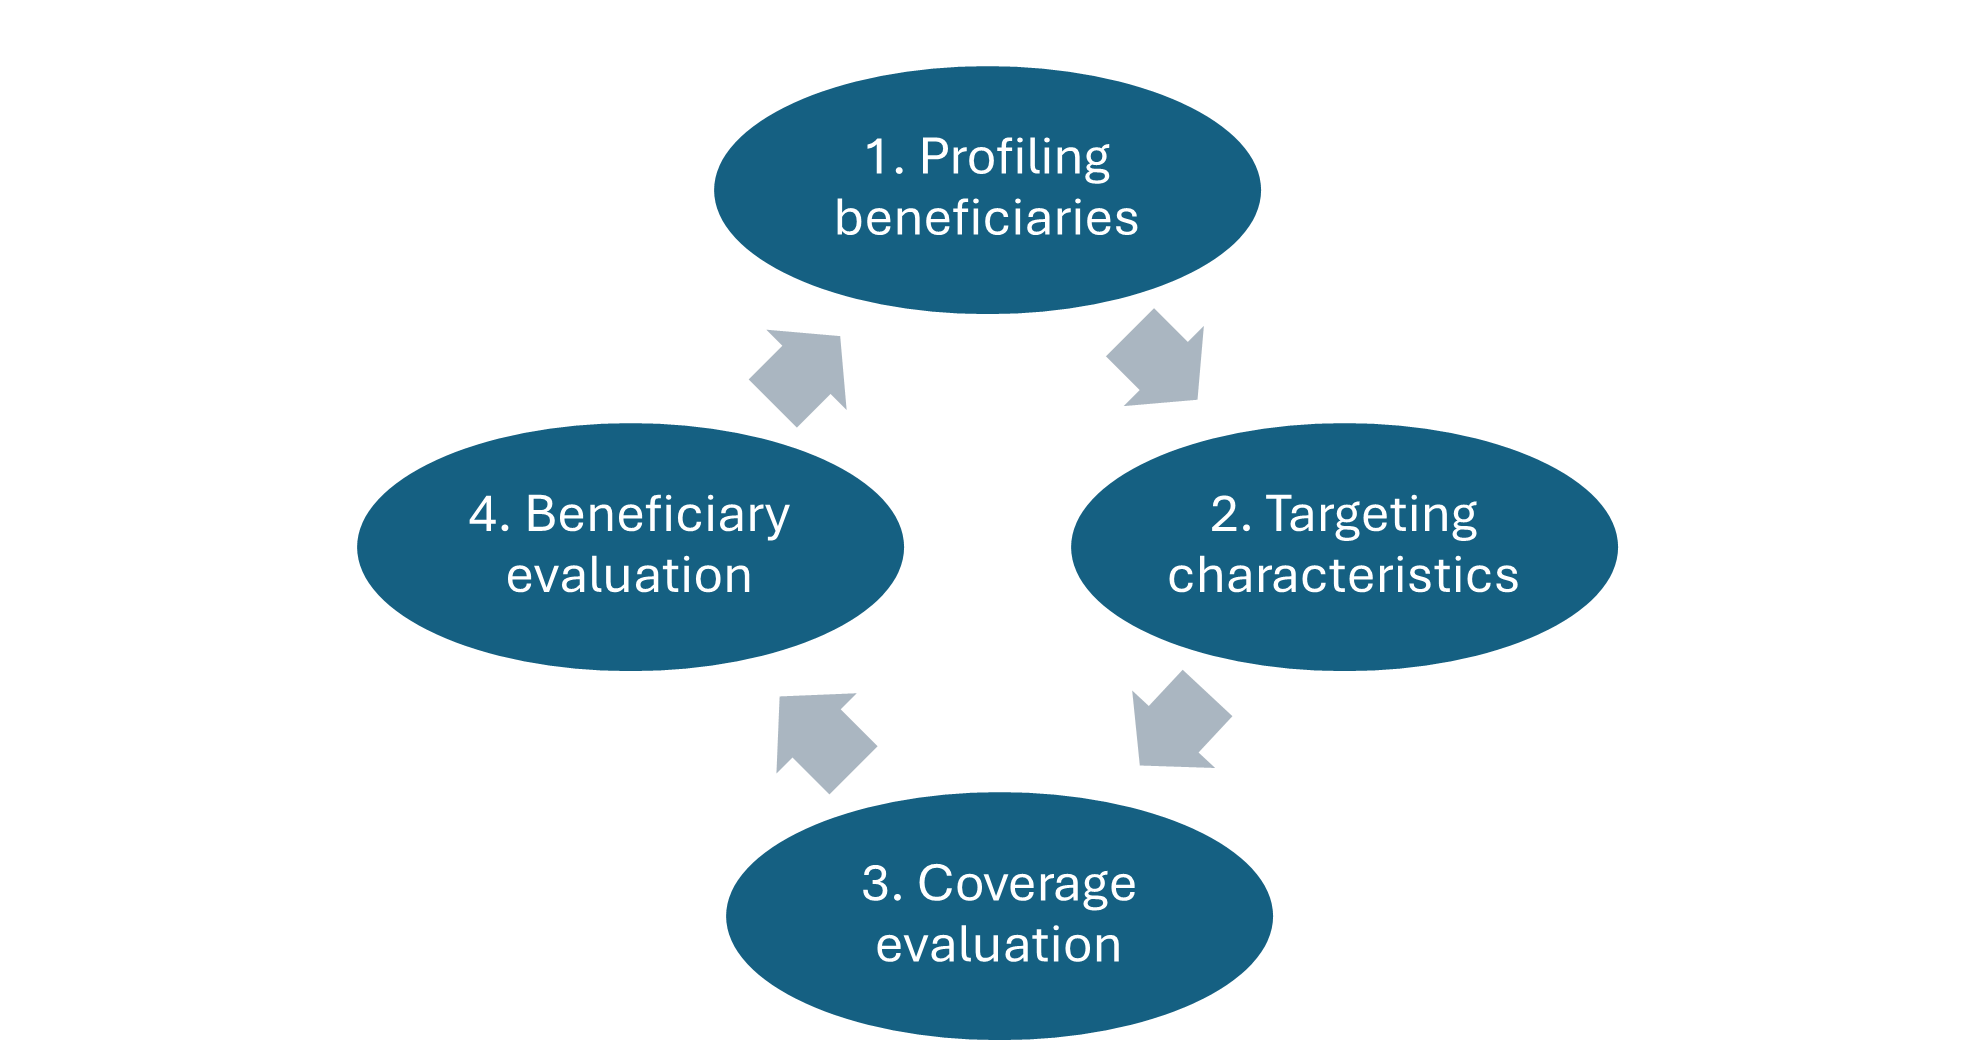
\includegraphics[keepaspectratio]{images/CH5.0_1.png}}

To maximize the practicality of the SPP-RAF, it has been built on four
pillars:

\begin{itemize}
\item
  \textbf{AI Use through Machine Learning Algorithms}: Machine learning
  algorithms are integrated into various stages of the process.
\item
  \textbf{Transparency}: The statistical techniques used to implement
  the SPP-RAF are:\\

  \begin{enumerate}
  \def\labelenumi{\alph{enumi}.}
  \tightlist
  \item
    \textbf{Replicable}: Results are independent of the individual
    performing the calculations.\\
  \item
    \textbf{Scalable}: The same tools can be used even as programmes
    expand their beneficiary numbers or coverage.\\
  \item
    \textbf{Standardized}: The same analytical procedures can be applied
    across different programmes.\\
  \item
    \textbf{Adaptable}: The analytical tools reflect changes in
    programme priorities and inform policymakers accordingly.
  \end{enumerate}
\item
  \textbf{Quantitative Analysis of Administrative Records}: The process
  relies on administrative records that are periodically updated as part
  of programme operations. This makes the analysis cost-effective, as no
  additional data collection is required. Moreover, the process is
  designed to start with minimal data requirements and expand as the
  social protection system matures. The conclusions drawn from the
  analysis reflect the local context, as they are based on data gathered
  from the programme.
\item
  \textbf{Evidence-Based Decisions}: Conclusions from the process are
  supported by data, ensuring transparency and strengthening the
  accountability and legitimacy of the organization. For example,
  policies derived from these conclusions can help policymakers justify
  their decisions in public debates by referencing the supporting data.
\item
  \textbf{Potential for Integration into Programme Operations}: Once
  institutionalized, the SPP-RAF can be used as a regular tool to
  monitor and assess programme progress. It has the potential to
  identify:\\

  \begin{enumerate}
  \def\labelenumi{\alph{enumi}.}
  \item
    Beneficiaries who have improved sufficiently to graduate from the
    programme.\\
  \item
    Applicants facing institutional or educational barriers to accessing
    the programme.\\
  \item
    Programmes with selection criteria that are no longer relevant, such
    as due to the existence of parallel programmes or schemes.\\
  \item
    Programmes whose target populations have shifted, such as an
    increase in young women entering the labour market and a decreased
    need for social assistance support.
  \end{enumerate}
\end{itemize}

\subsubsection{\texorpdfstring{\textbf{Context of the Programme to
Analyze}}{Context of the Programme to Analyze}}\label{context-of-the-programme-to-analyze}

Social assistance programmes, which are primarily non-contributory forms
of social protection, aim to alleviate poverty and vulnerability. Social
assistance is typically recognized through cash transfer programmes,
either unconditional or conditional, that provide monetary transfers to
target the most vulnerable households and/or individuals. Identifying
poverty and vulnerability, as evidenced by various measures of monetary
and multidimensional poverty, is one of the key challenges these
programmes face, as beneficiaries cannot self-select.

The programme under assessment for pedagogical purposes is a cash
transfer programme implemented in 2023 in the country of \textbf{Nemey}.
The Ministry of Social Solidarity has provided administrative records
for the first cohort of 2023, which includes data from 10,000 households
(with 43 household-level variables) and 46,360 individuals (with 24
individual-level variables). The collected data is essential for
calculating the Proxy Means Test (PMT), which assigns a score to each
household. This score determines eligibility for the programme.

\textbf{Context of the Information}

The dataset was gathered from a social protection programme in the
country of Nemey. It includes information from 10,000 households, each
with 43 variables, and data on 46,360 individuals, each with 24
variables.

\textbf{Key Variables in the Dataset:}

\begin{itemize}
\item
  \textbf{Relationship to Head of Household}: Values range from 1-9,
  representing different relationships such as head of the family,
  wife/husband, daughter/son, mother/father, etc.
\item
  \textbf{Gender}: Indicates the individual's gender, either ``Male'' or
  ``Female''.
\item
  \textbf{Date of Birth}: States the individual's age in years.
\item
  \textbf{Marital Status}: Specifies whether the individual is single,
  married, divorced, or widowed.
\item
  \textbf{School Attendance}: Indicates whether the individual is
  currently enrolled in school, has dropped out, never enrolled, or
  graduated.
\item
  \textbf{Schooling Level}: Describes the highest education level
  achieved, ranging from illiterate to university level.
\item
  \textbf{Chronic Disease}: Indicates if the individual suffers from
  diseases like cardiovascular disease, cancer, or kidney failure
  (Yes/No).
\item
  \textbf{Nutrition Disease}: Specifies if the individual suffers from
  permanent malnutrition, stunting, or wasting (Yes/No).
\item
  \textbf{Common Disease}: Indicates if the individual suffers from
  other diseases (e.g., measles, diphtheria, or polio) (Yes/No).
\item
  \textbf{Disability}: Categorized by severity: total disability (unable
  to perform chores independently), partial disability (able to work),
  or other disabilities (Yes/No).
\item
  \textbf{Health Insurance}: Indicates whether the individual has access
  to health insurance (Yes/No).
\item
  \textbf{Employment Status}: Describes the individual's employment
  status: employed, unemployed, or inactive.
\item
  \textbf{Job Type}: Specifies the individual's job type (e.g.,
  self-employed, paid in cash, paid in-kind, etc.).
\item
  \textbf{Contract Type}: Indicates the duration of the employment
  contract: permanent, temporary, seasonal, or not applicable.
\item
  \textbf{Employment Sector}: Specifies whether the individual works in
  the public or private sector (or does not apply if unemployed).
\item
  \textbf{Father Alive}: Indicates whether the individual's father is
  alive (Yes/No).
\end{itemize}

\textbf{Household Variables:}

\begin{itemize}
\item
  \textbf{Household Members}: The total number of members in the
  household.
\item
  \textbf{House Type}: Describes the type of housing (e.g., villa,
  independent modern house, apartment, farmwork/wood/zinc, etc.).
\item
  \textbf{Contract Type}: The dwelling ownership type (owned, rented,
  endowed, or other).
\item
  \textbf{House Size}: The size of the house in square meters.
\item
  \textbf{Number of Rooms}: The total number of rooms available for
  household members to sleep in.
\item
  \textbf{Wall/Floor/Roof Material}: Describes the materials used for
  the walls, roof, and floor.
\item
  \textbf{Wall/Floor/Roof Quality}: Indicates the level of damage to
  these structures, categorized from 1 (highest damage) to 3 (least
  damage).
\item
  \textbf{Cooking Fuel}: The type of fuel used for cooking (gas,
  kerosene, firewood/animal waste, etc.).
\item
  \textbf{Toilet Type}: Specifies if the toilet is an Arab toilet or a
  syringe and whether it is shared or not.
\item
  \textbf{Water and Electricity}: Specifies the sources of drinking
  water, water, electricity, and sewage water.
\item
  \textbf{Duration to Nearest Market/School/Hospital}: The time (in
  minutes) it takes to reach the nearest market, school, and/or
  hospital.
\item
  \textbf{Household Properties}: Indicates ownership of various
  household items (e.g., kitchen, TV, mobile phone, car, fridge, etc.).
\item
  \textbf{Livestock}: Indicates whether the household owns livestock
  (Yes/No).
\item
  \textbf{Agricultural Land}: Specifies the area of agricultural land
  owned by the household.
\item
  \textbf{Real Estate}: Indicates whether the household owns real estate
  (Yes/No).
\item
  \textbf{Governorate}: Nemey is divided into eight governorates,
  represented by the letters A-H, along with districts, municipalities,
  and villages/cities.
\item
  \textbf{Location}: Specifies if the household is located in an urban,
  rural, or remote area.
\end{itemize}

The government calculates a score based on the variables above, and
eligibility for the programme is determined by this score.

\subsection{\texorpdfstring{\textbf{1.Preparing the datasets of
Nemey}}{1.Preparing the datasets of Nemey}}\label{preparing-the-datasets-of-nemey}

The previous chapter delved into the details of connecting Excel and R
to produce rapid reports. This chapter implements these techniques
extensively to begin the generation of the SPP-RAF report. Keen readers
may wonder why this chapter is not included in Part 2. The reason is
that Part 2 is reserved for statistical techniques, while this chapter
serves as an introduction to that, i.e., producing relevant descriptive
statistics. Accordingly, this chapter, when placed in a report, can be
referred to as Chapter 0 or an introductory chapter. Here, the dataset
is described through graphs and tables, setting the stage for the
subsequent analysis. For this chapter, as well as for the following
chapters, the Excel files used are \texttt{DATA\_BASES.xlsx} and
\texttt{Beneficiaries.xlsx} (located in \texttt{Inputs/Data}) and
\texttt{Dictionary.xlsx} (located in \texttt{Inputs/Dictionary}).

\textbf{Full code available at:}
\href{https://github.com/ESCWASP/SPP_RAF}{Git hub SPP\_RAF}

Before starting any project, it is highly recommended to have an
organized folder structure. The suggested arrangement, as found in the
teaching aid material, includes separate folders for input, code, and
output. Once everything is organized, you can create an R project and
save it in the root folder (in the teaching aid, this project is named
SPP RAF.

A project, for practical purposes, is like a folder where you can group
multiple codes together. These codes are aware that they interact with
the same computer files. While you can work with individual scripts, as
we have done so far in the Master code \emph{SPP\_RAF\_full\_script.R},
splitting the code into manageable parts (e.g., chapters) is a good
practice for larger projects. This facilitates debugging and keeps the
code clean. In this context, the project serves as a powerful structure
that integrates these separate files through a well-synchronized master
file. Unlike other sections, several functions here are covered
superficially, as they do not significantly contribute to the reader's
general understanding, and their exact functionalities can be easily
found online.

\begin{Shaded}
\begin{Highlighting}[]
\FunctionTok{rm}\NormalTok{(}\AttributeTok{list =} \FunctionTok{ls}\NormalTok{())}
\FunctionTok{graphics.off}\NormalTok{()}
\FunctionTok{gc}\NormalTok{()}

\CommentTok{\# Paste start time}
\NormalTok{startTime  }\OtherTok{=} \FunctionTok{Sys.time}\NormalTok{()}
\end{Highlighting}
\end{Shaded}

The first four lines in the main script ensure that the software is
clean, with no graphs or variables saved from previous exercises. This
helps speed up calculations and avoids errors caused by previously
stored data. The last line acts as a time controller, recording when the
code begins to run. Later, at the end of the master file, a
complementary line records when the code stops running, allowing the
user to determine the duration of the process. This is particularly
useful for estimating running times and planning work accordingly. The
code below, for example, defines a list of R packages
(\texttt{myPackages}) commonly used for data manipulation,
visualization, statistical modeling, spatial analysis, and reporting. It
checks which packages are not installed and installs them with
dependencies. Then, it loads each package one by one, displaying a
message for each and handling any errors gracefully. If the
\texttt{extrafont} package is loaded and the system is Windows, it loads
fonts for better plotting, particularly, as we are using Arabic as our
second language.

\begin{Shaded}
\begin{Highlighting}[]

\CommentTok{\# 1| Preparation {-}{-}{-}{-}{-}{-}{-}{-}{-}{-}{-}{-}{-}{-}{-}{-}{-}{-}{-}{-}{-}{-}{-}{-}{-}{-}{-}{-}{-}{-}{-}{-}{-}{-}{-}{-}{-}{-}{-}{-}{-}{-}{-}{-}{-}{-}{-}{-}{-}{-}{-}{-}{-}{-}{-}{-}}
\CommentTok{\# 1.1| Libraries {-}{-}{-}{-}{-}{-}{-}{-}{-}{-}{-}{-}{-}{-}{-}{-}{-}{-}{-}{-}{-}{-}{-}{-}{-}{-}{-}{-}{-}{-}{-}{-}{-}{-}{-}{-}{-}{-}{-}{-}{-}{-}{-}{-}{-}{-}{-}{-}{-}{-}{-}{-}{-}{-}{-}{-}}
\CommentTok{\# List of packages}
\NormalTok{myPackages }\OtherTok{\textless{}{-}} \FunctionTok{c}\NormalTok{(}
  \StringTok{\textquotesingle{}broom\textquotesingle{}}\NormalTok{,}\StringTok{\textquotesingle{}caret\textquotesingle{}}\NormalTok{,}\StringTok{\textquotesingle{}cluster\textquotesingle{}}\NormalTok{,}\StringTok{\textquotesingle{}clValid\textquotesingle{}}\NormalTok{,}\StringTok{\textquotesingle{}cobalt\textquotesingle{}}\NormalTok{,}\StringTok{\textquotesingle{}colorspace\textquotesingle{}}\NormalTok{,}\StringTok{\textquotesingle{}data.table\textquotesingle{}}\NormalTok{,}\StringTok{\textquotesingle{}descr\textquotesingle{}}\NormalTok{,}
  \StringTok{\textquotesingle{}dplyr\textquotesingle{}}\NormalTok{,}\StringTok{\textquotesingle{}extrafont\textquotesingle{}}\NormalTok{,}\StringTok{\textquotesingle{}factoextra\textquotesingle{}}\NormalTok{,}\StringTok{\textquotesingle{}FactoMineR\textquotesingle{}}\NormalTok{,}\StringTok{\textquotesingle{}fastDummies\textquotesingle{}}\NormalTok{,}\StringTok{\textquotesingle{}foreign\textquotesingle{}}\NormalTok{,}\StringTok{\textquotesingle{}fpc\textquotesingle{}}\NormalTok{,}\StringTok{\textquotesingle{}gbm\textquotesingle{}}\NormalTok{,}
  \StringTok{\textquotesingle{}geosphere\textquotesingle{}}\NormalTok{,}\StringTok{\textquotesingle{}ggdendro\textquotesingle{}}\NormalTok{,}\StringTok{\textquotesingle{}ggparty\textquotesingle{}}\NormalTok{,}\StringTok{\textquotesingle{}ggplot2\textquotesingle{}}\NormalTok{,}\StringTok{\textquotesingle{}ggpubr\textquotesingle{}}\NormalTok{,}\StringTok{\textquotesingle{}ggspatial\textquotesingle{}}\NormalTok{,}\StringTok{\textquotesingle{}ggmap\textquotesingle{}}\NormalTok{,}\StringTok{\textquotesingle{}glmnet\textquotesingle{}}\NormalTok{,}
  \StringTok{\textquotesingle{}gridExtra\textquotesingle{}}\NormalTok{,}\StringTok{\textquotesingle{}gtools\textquotesingle{}}\NormalTok{,}\StringTok{\textquotesingle{}haven\textquotesingle{}}\NormalTok{,}\StringTok{\textquotesingle{}here\textquotesingle{}}\NormalTok{,}\StringTok{\textquotesingle{}Hmisc\textquotesingle{}}\NormalTok{,}\StringTok{\textquotesingle{}igraph\textquotesingle{}}\NormalTok{,}\StringTok{\textquotesingle{}Metrics\textquotesingle{}}\NormalTok{,}\StringTok{\textquotesingle{}openxlsx\textquotesingle{}}\NormalTok{,}\StringTok{\textquotesingle{}partykit\textquotesingle{}}\NormalTok{,}
  \StringTok{\textquotesingle{}PCAmixdata\textquotesingle{}}\NormalTok{,}\StringTok{\textquotesingle{}ppcor\textquotesingle{}}\NormalTok{,}\StringTok{\textquotesingle{}purrr\textquotesingle{}}\NormalTok{,}\StringTok{\textquotesingle{}questionr\textquotesingle{}}\NormalTok{,}\StringTok{\textquotesingle{}raster\textquotesingle{}}\NormalTok{,}\StringTok{\textquotesingle{}RColorBrewer\textquotesingle{}}\NormalTok{,}\StringTok{\textquotesingle{}readr\textquotesingle{}}\NormalTok{,}\StringTok{\textquotesingle{}readxl\textquotesingle{}}\NormalTok{,}
  \StringTok{\textquotesingle{}reshape2\textquotesingle{}}\NormalTok{,}\StringTok{\textquotesingle{}rpart\textquotesingle{}}\NormalTok{,}\StringTok{\textquotesingle{}rpart.plot\textquotesingle{}}\NormalTok{,}\StringTok{\textquotesingle{}scales\textquotesingle{}}\NormalTok{,}\StringTok{\textquotesingle{}sf\textquotesingle{}}\NormalTok{,}\StringTok{\textquotesingle{}shadowtext\textquotesingle{}}\NormalTok{,}\StringTok{\textquotesingle{}spatstat\textquotesingle{}}\NormalTok{,}\StringTok{\textquotesingle{}stars\textquotesingle{}}\NormalTok{,}
  \StringTok{\textquotesingle{}StatMatch\textquotesingle{}}\NormalTok{,}\StringTok{\textquotesingle{}stringr\textquotesingle{}}\NormalTok{,}\StringTok{\textquotesingle{}survey\textquotesingle{}}\NormalTok{,}\StringTok{\textquotesingle{}tidyr\textquotesingle{}}\NormalTok{,}\StringTok{\textquotesingle{}tidyverse\textquotesingle{}}\NormalTok{,}\StringTok{\textquotesingle{}treemapify\textquotesingle{}}\NormalTok{,}\StringTok{\textquotesingle{}writexl\textquotesingle{}}\NormalTok{,}\StringTok{\textquotesingle{}eeptools\textquotesingle{}}\NormalTok{,}
  \StringTok{\textquotesingle{}lubridate\textquotesingle{}}\NormalTok{,}\StringTok{\textquotesingle{}lattice\textquotesingle{}}\NormalTok{,}\StringTok{\textquotesingle{}sfsmisc\textquotesingle{}}
\NormalTok{)}

\CommentTok{\# Identify missing packages}
\NormalTok{notInstalled }\OtherTok{\textless{}{-}}\NormalTok{ myPackages[}\SpecialCharTok{!}\NormalTok{(myPackages }\SpecialCharTok{\%in\%} \FunctionTok{rownames}\NormalTok{(}\FunctionTok{installed.packages}\NormalTok{()))]}

\CommentTok{\# Install missing packages with dependencies}
\ControlFlowTok{if}\NormalTok{ (}\FunctionTok{length}\NormalTok{(notInstalled)) \{}
  \FunctionTok{install.packages}\NormalTok{(notInstalled, }\AttributeTok{dependencies =} \ConstantTok{TRUE}\NormalTok{)}
\NormalTok{\}}

\CommentTok{\# Load packages one{-}by{-}one with feedback}
\ControlFlowTok{for}\NormalTok{ (pkg }\ControlFlowTok{in}\NormalTok{ myPackages) \{}
  \FunctionTok{message}\NormalTok{(}\StringTok{"Loading: "}\NormalTok{, pkg)}
  \FunctionTok{tryCatch}\NormalTok{(\{}
    \FunctionTok{library}\NormalTok{(pkg, }\AttributeTok{character.only =} \ConstantTok{TRUE}\NormalTok{, }\AttributeTok{quietly =} \ConstantTok{TRUE}\NormalTok{)}
\NormalTok{  \}, }\AttributeTok{error =} \ControlFlowTok{function}\NormalTok{(e) \{}
    \FunctionTok{warning}\NormalTok{(}\StringTok{"Failed to load package: "}\NormalTok{, pkg, }\StringTok{"}\SpecialCharTok{\textbackslash{}n}\StringTok{"}\NormalTok{, e}\SpecialCharTok{$}\NormalTok{message)}
\NormalTok{  \})}
\NormalTok{\}}

\CommentTok{\# Load fonts only if extrafont is available and on Windows}
\ControlFlowTok{if}\NormalTok{ (}\StringTok{"extrafont"} \SpecialCharTok{\%in\%} \FunctionTok{loadedNamespaces}\NormalTok{() }\SpecialCharTok{\&\&}\NormalTok{ .Platform}\SpecialCharTok{$}\NormalTok{OS.type }\SpecialCharTok{==} \StringTok{"windows"}\NormalTok{) \{}
  \FunctionTok{try}\NormalTok{(}\FunctionTok{loadfonts}\NormalTok{(}\AttributeTok{device =} \StringTok{"win"}\NormalTok{, }\AttributeTok{quiet =} \ConstantTok{TRUE}\NormalTok{), }\AttributeTok{silent =} \ConstantTok{TRUE}\NormalTok{)}
\NormalTok{\}}

\CommentTok{\# Disable scientific notation}
\FunctionTok{options}\NormalTok{(}\AttributeTok{scipen =} \DecValTok{999}\NormalTok{)}


\CommentTok{\# 1.2| Initial values locations and folders}
\CommentTok{\# 1: English.}
\CommentTok{\# 0: Arabic.}
\NormalTok{language }\OtherTok{=} \DecValTok{0}

\CommentTok{\# Specify location of file}
\NormalTok{userLocation   }\OtherTok{=} \FunctionTok{enc2native}\NormalTok{(}\FunctionTok{here}\NormalTok{()) }\CommentTok{\# Replace by your own path.}

\DocumentationTok{\#\# Create output folders if not available to save the output}
\ControlFlowTok{if}\NormalTok{(}\SpecialCharTok{!}\FunctionTok{file.exists}\NormalTok{(}\StringTok{"Output"}\NormalTok{))\{}
  \FunctionTok{dir.create}\NormalTok{(}\StringTok{"Output"}\NormalTok{)  }
\NormalTok{\}}
\ControlFlowTok{if}\NormalTok{(}\SpecialCharTok{!}\FunctionTok{file.exists}\NormalTok{(}\StringTok{"Output/Clustering"}\NormalTok{))\{}
  \FunctionTok{dir.create}\NormalTok{(}\StringTok{"Output/Clustering"}\NormalTok{)  }
\NormalTok{\}}
\ControlFlowTok{if}\NormalTok{(}\SpecialCharTok{!}\FunctionTok{file.exists}\NormalTok{(}\StringTok{"Output/Targeting Assessment"}\NormalTok{))\{}
  \FunctionTok{dir.create}\NormalTok{(}\StringTok{"Output/Targeting Assessment"}\NormalTok{)  }
\NormalTok{\}}
\ControlFlowTok{if}\NormalTok{(}\SpecialCharTok{!}\FunctionTok{file.exists}\NormalTok{(}\StringTok{"Output/Coverage Evaluation"}\NormalTok{))\{}
  \FunctionTok{dir.create}\NormalTok{(}\StringTok{"Output/Coverage Evaluation"}\NormalTok{)  }
\NormalTok{\}}
\CommentTok{\# Location of Input and Code folders}
\NormalTok{scriptLocation }\OtherTok{=} \FunctionTok{paste0}\NormalTok{(userLocation, }\StringTok{\textquotesingle{}/Code/\textquotesingle{}}\NormalTok{)}
\NormalTok{inputLocation  }\OtherTok{=} \FunctionTok{paste0}\NormalTok{(userLocation, }\StringTok{\textquotesingle{}/Input/\textquotesingle{}}\NormalTok{)}
\end{Highlighting}
\end{Shaded}

\paragraph{\texorpdfstring{\textbf{Updating main datasets: Individual
and Household
Data}}{Updating main datasets: Individual and Household Data}}\label{updating-main-datasets-individual-and-household-data}

As previously noted, the programme selected for evaluation, for
pedagogical purposes, is a Cash Transfer Programme implemented in the
country of Nemey since 2023. The datasets analyzed comprise information
on 10,000 households (43 variables) and 46,360 individuals (24
variables). All variables collected are essential for the Proxy Means
Test (PMT), which, once estimated for each household, will generate a
score of which will be discussed in the following sections.

\begin{Shaded}
\begin{Highlighting}[]
\DocumentationTok{\#\#1.3 Uploading main datasets: Individual and Household Data  {-}{-}{-}{-}{-}{-}{-}{-}{-}{-}{-}{-}{-}{-}{-}{-}{-}{-}{-}{-}{-}{-}{-}{-}{-}{-}{-}{-}{-}{-}{-}{-}{-}{-}{-}{-}{-}{-}{-}{-}{-}{-}{-}{-}{-}{-}{-}{-}{-}{-}{-}}
\NormalTok{IndividualData}\OtherTok{=}\FunctionTok{read\_excel}\NormalTok{(}\FunctionTok{paste0}\NormalTok{(inputLocation, }\StringTok{\textquotesingle{}Bases/DATA\_BASES.xlsx\textquotesingle{}}\NormalTok{), }\AttributeTok{sheet =} \StringTok{\textquotesingle{}Individuals\textquotesingle{}}\NormalTok{,}\AttributeTok{na =} \StringTok{"NULL"}\NormalTok{)}
\NormalTok{HH\_Data}\OtherTok{=}\FunctionTok{read\_excel}\NormalTok{(}\FunctionTok{paste0}\NormalTok{(inputLocation, }\StringTok{\textquotesingle{}Bases/DATA\_BASES.xlsx\textquotesingle{}}\NormalTok{), }\AttributeTok{sheet =} \StringTok{\textquotesingle{}Households\textquotesingle{}}\NormalTok{,}\AttributeTok{na =} \StringTok{"NULL"}\NormalTok{)}

\NormalTok{IndividualData }\OtherTok{=}\NormalTok{ IndividualData }\SpecialCharTok{\%\textgreater{}\%} 
  \FunctionTok{mutate}\NormalTok{(}\StringTok{\textasciigrave{}}\AttributeTok{Schooling level}\StringTok{\textasciigrave{}}\OtherTok{=}\FunctionTok{if\_else}\NormalTok{(}\StringTok{\textasciigrave{}}\AttributeTok{Schooling level}\StringTok{\textasciigrave{}}\SpecialCharTok{\%in\%}\FunctionTok{c}\NormalTok{(}\StringTok{"illiterat"}\NormalTok{), }\StringTok{"illiterate"}\NormalTok{,}\StringTok{\textasciigrave{}}\AttributeTok{Schooling level}\StringTok{\textasciigrave{}}\NormalTok{))}

\NormalTok{IndividualData }\OtherTok{=}\NormalTok{ IndividualData }\SpecialCharTok{\%\textgreater{}\%}
  \FunctionTok{mutate}\NormalTok{(}\AttributeTok{Age =} \FunctionTok{trunc}\NormalTok{((}\FunctionTok{as.Date}\NormalTok{(}\StringTok{\textasciigrave{}}\AttributeTok{Date of birth}\StringTok{\textasciigrave{}}\NormalTok{) }\SpecialCharTok{\%{-}{-}\%} \FunctionTok{as.Date}\NormalTok{(}\FunctionTok{Sys.Date}\NormalTok{()) }\SpecialCharTok{/} \FunctionTok{years}\NormalTok{(}\DecValTok{1}\NormalTok{) )))}
\end{Highlighting}
\end{Shaded}

\paragraph{Dictionary Uses and Calls in the
Code}\label{dictionary-uses-and-calls-in-the-code}

The Dictionary is a key feature that supports the cleaning and
standardization of datasets, particularly when variable labels are not
clear and/or require translation. The dictionary provided for these
exercises contains three sheets, which will be described in detail,
along with an example code snippet demonstrating how to read and upload
it in R. The three sheets are:

\begin{enumerate}
\def\labelenumi{\arabic{enumi}.}
\tightlist
\item
  \textbf{Labels}: This sheet contains all the titles, subtitles,
  legends for X and Y axes for all the plots in English and Arabic.
\end{enumerate}

\begin{Shaded}
\begin{Highlighting}[]
\CommentTok{\# 1.4 Uploading dictionary {-} Labels  {-}{-}{-}{-}{-}{-}{-}{-}{-}{-}{-}{-}{-}{-}{-}{-}{-}{-}{-}{-}{-}{-}{-}{-}{-}{-}{-}{-}{-}{-}{-}{-}{-}{-}{-}{-}{-}{-}{-}{-}{-}{-}{-}{-}{-}{-}{-}{-}{-}{-}{-}}
\NormalTok{dataPlots }\OtherTok{\textless{}{-}} \FunctionTok{read\_excel}\NormalTok{(}\FunctionTok{paste0}\NormalTok{(inputLocation, }\StringTok{\textquotesingle{}Dictionary/Dictionary.xlsx\textquotesingle{}}\NormalTok{), }
                        \AttributeTok{sheet =} \StringTok{\textquotesingle{}Labels\textquotesingle{}}\NormalTok{)}
\NormalTok{dataPlots[}\FunctionTok{is.na}\NormalTok{(dataPlots)] }\OtherTok{\textless{}{-}} \StringTok{\textquotesingle{}\textquotesingle{}} \CommentTok{\# Replace NAs with characters}
\end{Highlighting}
\end{Shaded}

\begin{enumerate}
\def\labelenumi{\arabic{enumi}.}
\setcounter{enumi}{1}
\tightlist
\item
  \textbf{Category}: This sheet provides a correspondence table linking
  household and individual variables with their names in both English
  and Arabic. It also includes the levels of categorical variables, such
  as gender (Male or Female) and all variables with Yes/No categories.
\end{enumerate}

\begin{Shaded}
\begin{Highlighting}[]
\CommentTok{\# 1.5 Uploading Dictionary {-} Category {-}{-}{-}{-}{-}{-}{-}{-}{-}{-}{-}{-}{-}{-}{-}{-}{-}{-}{-}{-}{-}{-}{-}{-}{-}{-}{-}{-}{-}{-}{-}{-}{-}{-}{-}{-}{-}{-}{-}{-}{-}{-}{-}{-}{-}{-}{-}{-}{-}{-}{-}{-}{-}{-}}
\CommentTok{\# Referring each graph to its specific labels in the dictionary}
\NormalTok{IndVarNames }\OtherTok{\textless{}{-}} \FunctionTok{as.matrix}\NormalTok{(}\FunctionTok{read\_excel}\NormalTok{(}\FunctionTok{paste0}\NormalTok{(inputLocation, }\StringTok{\textquotesingle{}Dictionary/Dictionary.xlsx\textquotesingle{}}\NormalTok{), }\AttributeTok{sheet =} \StringTok{\textquotesingle{}Category\textquotesingle{}}\NormalTok{, }\AttributeTok{range =} \StringTok{\textquotesingle{}A8:D32\textquotesingle{}}\NormalTok{)) }
\NormalTok{HHVarNames }\OtherTok{\textless{}{-}} \FunctionTok{as.matrix}\NormalTok{(}\FunctionTok{read\_excel}\NormalTok{(}\FunctionTok{paste0}\NormalTok{(inputLocation, }\StringTok{\textquotesingle{}Dictionary/Dictionary.xlsx\textquotesingle{}}\NormalTok{), }\AttributeTok{sheet =} \StringTok{\textquotesingle{}Category\textquotesingle{}}\NormalTok{, }\AttributeTok{range =} \StringTok{\textquotesingle{}F8:I51\textquotesingle{}}\NormalTok{)) }

\NormalTok{GenderLabels }\OtherTok{\textless{}{-}} \FunctionTok{as.matrix}\NormalTok{(}\FunctionTok{read\_excel}\NormalTok{(}\FunctionTok{paste0}\NormalTok{(inputLocation, }\StringTok{\textquotesingle{}Dictionary/Dictionary.xlsx\textquotesingle{}}\NormalTok{), }\AttributeTok{sheet =} \StringTok{\textquotesingle{}Category\textquotesingle{}}\NormalTok{, }\AttributeTok{range =} \StringTok{\textquotesingle{}A1:D3\textquotesingle{}}\NormalTok{)) }

\NormalTok{YesNoLabels }\OtherTok{\textless{}{-}} \FunctionTok{as.matrix}\NormalTok{(}\FunctionTok{read\_excel}\NormalTok{(}\FunctionTok{paste0}\NormalTok{(inputLocation, }\StringTok{\textquotesingle{}Dictionary/Dictionary.xlsx\textquotesingle{}}\NormalTok{), }\AttributeTok{sheet =} \StringTok{\textquotesingle{}Category\textquotesingle{}}\NormalTok{, }\AttributeTok{range =} \StringTok{\textquotesingle{}F1:I3\textquotesingle{}}\NormalTok{)) }
\end{Highlighting}
\end{Shaded}

\begin{enumerate}
\def\labelenumi{\arabic{enumi}.}
\setcounter{enumi}{2}
\tightlist
\item
  \textbf{Weights of the variable's categories}: According to the PMT
  (which will be explained later in Chapter 6), every variable of the
  social registry and their category has a weight according to the
  formula defined by the hypothetical case of the Nemey country. Many
  variables are based on observable characteristics of the housing. For
  example, if a house has cement walls without modest damage (weight is
  20 in the Dictionary), the weight will be lower if the house has walls
  of wood with significant damages (weight is 90 in the Dictionary).
  Below is a chunk of code uploading the variables
  \texttt{Dwelling\ Type} and \texttt{Wall\ Type}. This format will
  definitely change according to the weights format, variables,
  iterations, among others, so this code is only indicative to follow
  the full example provided.
\end{enumerate}

\begin{Shaded}
\begin{Highlighting}[]
\DocumentationTok{\#\# 1.6 Uploading Dictionary {-} Weights}
\NormalTok{DwellingTypeWeights }\OtherTok{\textless{}{-}} \FunctionTok{read\_excel}\NormalTok{(}\FunctionTok{paste0}\NormalTok{(inputLocation, }\StringTok{\textquotesingle{}Dictionary/Dictionary.xlsx\textquotesingle{}}\NormalTok{), }\AttributeTok{sheet =} \StringTok{\textquotesingle{}Weights\textquotesingle{}}\NormalTok{, }\AttributeTok{range =} \StringTok{\textquotesingle{}A2:C46\textquotesingle{}}\NormalTok{) }\SpecialCharTok{\%\textgreater{}\%}  \CommentTok{\#from to}
  \FunctionTok{rename}\NormalTok{(}\StringTok{\textasciigrave{}}\AttributeTok{House type}\StringTok{\textasciigrave{}}\OtherTok{=}\NormalTok{Dwelling\_type, }\StringTok{\textasciigrave{}}\AttributeTok{Contract type}\StringTok{\textasciigrave{}}\OtherTok{=}\NormalTok{ Dwelling\_ownership, }\AttributeTok{var\_Dwelling\_type=}\NormalTok{weight)}
\NormalTok{WallTypeWeights }\OtherTok{\textless{}{-}} \FunctionTok{read\_excel}\NormalTok{(}\FunctionTok{paste0}\NormalTok{(inputLocation, }\StringTok{\textquotesingle{}Dictionary/Dictionary.xlsx\textquotesingle{}}\NormalTok{), }\AttributeTok{sheet =} \StringTok{\textquotesingle{}Weights\textquotesingle{}}\NormalTok{, }\AttributeTok{range =} \StringTok{\textquotesingle{}E2:G20\textquotesingle{}}\NormalTok{)}\SpecialCharTok{\%\textgreater{}\%} \CommentTok{\#from to}
  \FunctionTok{rename}\NormalTok{(}\StringTok{\textasciigrave{}}\AttributeTok{Wall material}\StringTok{\textasciigrave{}}\OtherTok{=}\NormalTok{Wall\_type, }\StringTok{\textasciigrave{}}\AttributeTok{Wall quality}\StringTok{\textasciigrave{}}\OtherTok{=}\NormalTok{ Damage\_level, }\AttributeTok{var\_Wall\_type=}\NormalTok{weight)}
\end{Highlighting}
\end{Shaded}

\paragraph{Updating names of columns and categories in the
datasets}\label{updating-names-of-columns-and-categories-in-the-datasets}

Once the dictionaries are loaded, the datasets must be transformed by
replacing the names of variables that might not be clear with the full
names provided in the dictionary. Similarly, categorical data should be
converted into factors for proper analysis.

\begin{Shaded}
\begin{Highlighting}[]
\CommentTok{\# 1.7| Renaming variables in each dataset}
\SpecialCharTok{{-}{-}{-}{-}{-}{-}{-}{-}{-}{-}{-}{-}{-}{-}{-}{-}{-}{-}{-}{-}{-}{-}{-}{-}{-}{-}{-}{-}{-}{-}{-}{-}{-}{-}{-}{-}{-}{-}{-}{-}{-}{-}{-}{-}{-}{-}{-}{-}{-}{-}{-}{-}{-}{-}}
\FunctionTok{colnames}\NormalTok{(IndividualData) }\OtherTok{=} \FunctionTok{as.character}\NormalTok{(}\FunctionTok{factor}\NormalTok{(}\FunctionTok{colnames}\NormalTok{(IndividualData),}
                                          \AttributeTok{levels =}\NormalTok{ IndVarNames[,}\DecValTok{2}\NormalTok{],}
                                          \AttributeTok{labels =}\NormalTok{ IndVarNames[,}\DecValTok{4{-}1}\NormalTok{]))}
\FunctionTok{colnames}\NormalTok{(HH\_Data) }\OtherTok{=} \FunctionTok{as.character}\NormalTok{(}\FunctionTok{factor}\NormalTok{(}\FunctionTok{colnames}\NormalTok{(HH\_Data),}
                                      \AttributeTok{levels =}\NormalTok{ HHVarNames[,}\DecValTok{2}\NormalTok{],}
                                      \AttributeTok{labels =}\NormalTok{ HHVarNames[,}\DecValTok{4{-}1}\NormalTok{]))}
\NormalTok{HH\_Data }\OtherTok{=}\NormalTok{ HH\_Data[,}\SpecialCharTok{!}\FunctionTok{is.na}\NormalTok{(}\FunctionTok{colnames}\NormalTok{(HH\_Data))]}

\CommentTok{\# 1.10 Convert categorical variables of individuals dataset into factors. 1.10 section repeats the process for the househol ddataset }
\SpecialCharTok{{-}{-}{-}{-}{-}{-}{-}{-}{-}{-}{-}{-}{-}{-}{-}{-}{-}{-}{-}{-}{-}{-}{-}{-}{-}{-}{-}{-}{-}{-}{-}{-}{-}{-}{-}{-}{-}{-}{-}{-}{-}{-}{-}{-}{-}{-}{-}{-}{-}{-}{-}{-}{-}{-}}
\CommentTok{\# Also, in case another language wants to be used as a label for the data, this code will update to the language selected (in this case, language 1 is English, 0 is Arabic).}

\NormalTok{Individual\_Data}\SpecialCharTok{$}\StringTok{\textasciigrave{}}\AttributeTok{Gender}\StringTok{\textasciigrave{}} \OtherTok{=} \FunctionTok{as.character}\NormalTok{(}\FunctionTok{factor}\NormalTok{(Individual\_Data}\SpecialCharTok{$}\StringTok{\textasciigrave{}}\AttributeTok{Gender}\StringTok{\textasciigrave{}}\NormalTok{,}
                                  \AttributeTok{levels =}\NormalTok{ GenderLabels[,}\DecValTok{2}\NormalTok{],}
                                  \AttributeTok{labels =}\NormalTok{ GenderLabels[,}\DecValTok{4}\SpecialCharTok{{-}}\NormalTok{language]))}
\NormalTok{Individual\_Data}\SpecialCharTok{$}\StringTok{\textasciigrave{}}\AttributeTok{School attendance}\StringTok{\textasciigrave{}} \OtherTok{=} \FunctionTok{as.character}\NormalTok{(}\FunctionTok{factor}\NormalTok{(Individual\_Data}\SpecialCharTok{$}\StringTok{\textasciigrave{}}\AttributeTok{School attendance}\StringTok{\textasciigrave{}}\NormalTok{,}
                              \AttributeTok{levels =}\NormalTok{ EducationAttainment[,}\DecValTok{2}\NormalTok{],}
                              \AttributeTok{labels =}\NormalTok{ EducationAttainment[,}\DecValTok{4}\SpecialCharTok{{-}}\NormalTok{language]))}
\end{Highlighting}
\end{Shaded}

\paragraph{Vulnerability variables: Creation of new variables from
Individual to Household
datasets}\label{vulnerability-variables-creation-of-new-variables-from-individual-to-household-datasets}

Based on individual characteristics, household-level variables can be
created to capture information such as the household illiteracy rate,
the presence of NEET members (Not in Education, Employment, or
Training), or whether there are children out of school. These
transformations involve multiple steps. For pedagogical purposes, we
will demonstrate the process for calculating the household illiteracy
rate. However, reviewing the complete code is essential for a full
understanding in the section 1.8 and 1.9

\begin{Shaded}
\begin{Highlighting}[]
\CommentTok{\# Example Creation of Relevant Variables from Individual to Household Datasets}
\SpecialCharTok{{-}{-}{-}{-}{-}{-}{-}{-}{-}{-}{-}{-}{-}{-}{-}{-}{-}{-}{-}{-}{-}{-}{-}{-}{-}{-}{-}{-}{-}{-}{-}{-}{-}{-}{-}{-}{-}{-}{-}{-}{-}{-}{-}{-}{-}{-}{-}{-}{-}{-}{-}{-}{-}{-}}
\NormalTok{Test\_Iliteracy\_rate }\OtherTok{=}\NormalTok{ IndividualData }\SpecialCharTok{\%\textgreater{}\%} \FunctionTok{group\_by}\NormalTok{(HHID) }\SpecialCharTok{\%\textgreater{}\%}
  \FunctionTok{mutate}\NormalTok{(}\AttributeTok{illiterate =} \FunctionTok{if\_else}\NormalTok{(Age }\SpecialCharTok{\textgreater{}} \DecValTok{15} \SpecialCharTok{\&} \StringTok{\textasciigrave{}}\AttributeTok{Schooling level}\StringTok{\textasciigrave{}} \SpecialCharTok{\%in\%} \FunctionTok{c}\NormalTok{(}\StringTok{"illiterate"}\NormalTok{), }\DecValTok{1}\NormalTok{, }\DecValTok{0}\NormalTok{),}
         \AttributeTok{members\_15above =} \FunctionTok{if\_else}\NormalTok{(Age }\SpecialCharTok{\textgreater{}} \DecValTok{15}\NormalTok{, }\DecValTok{1}\NormalTok{, }\DecValTok{0}\NormalTok{)) }\SpecialCharTok{\%\textgreater{}\%}
  \FunctionTok{summarise}\NormalTok{(}\AttributeTok{var\_illiteracy\_rate =} \DecValTok{100} \SpecialCharTok{*} \FunctionTok{sum}\NormalTok{(illiterate) }\SpecialCharTok{/}\NormalTok{ (}\FunctionTok{sum}\NormalTok{(members\_15above))) }\SpecialCharTok{\%\textgreater{}\%}
  \FunctionTok{mutate}\NormalTok{(}\AttributeTok{var\_illiteracy\_rate =} \FunctionTok{if\_else}\NormalTok{(}\FunctionTok{is.nan}\NormalTok{(var\_illiteracy\_rate), }\DecValTok{100}\NormalTok{, var\_illiteracy\_rate))}
\end{Highlighting}
\end{Shaded}

\subsection{2. PMT and Scoring
Estimations}\label{pmt-and-scoring-estimations}

To address self-selection, many countries first select beneficiaries
based on observable criteria such as age or disability, then conduct
social surveys to comprehensively assess the socioeconomic status of
household members. This evaluation is converted into a set of observable
variables that proxy the level of poverty or vulnerability of the
households. Based on statistical exercises, each variable has a certain
``relevance'' when explaining poverty or vulnerability. For example,
owning a house with a roof made of brick or asbestos is less important
in explaining vulnerability compared to the employment status of the
head of the household. While both variables can explain vulnerability to
some extent, the employment status is one of the most relevant factors.
The combination of variables and weights assigns a score to applicants
or selected households, which ranks and determines their relative level
of vulnerability.

\subsubsection{2.1 Link the PMT weights with the Variables'
categories}\label{link-the-pmt-weights-with-the-variables-categories}

The weights of the variables were explained earlier in the chapter,
particularly for non-binary variables such as wall type (iterated by
damage) or dwelling property type (weights of the variable's
categories). For binary variables, such as car ownership (1 or 0), the
weights are determined in the code: 10 for households without a bike and
0 for those with a car.

\begin{Shaded}
\begin{Highlighting}[]
\CommentTok{\#Example, full code in section 1.8}
\SpecialCharTok{{-}{-}{-}{-}{-}{-}{-}{-}{-}{-}{-}{-}{-}{-}{-}{-}{-}{-}{-}{-}{-}{-}{-}{-}{-}{-}{-}{-}{-}{-}{-}{-}{-}{-}{-}{-}{-}{-}{-}{-}{-}{-}{-}{-}{-}{-}{-}{-}{-}{-}{-}{-}{-}{-}}
\NormalTok{Indicators\_example }\OtherTok{=}\NormalTok{ HH\_Data }\SpecialCharTok{\%\textgreater{}\%}
  \FunctionTok{left\_join}\NormalTok{(DwellingTypeWeights) }\SpecialCharTok{\%\textgreater{}\%} 
  \FunctionTok{left\_join}\NormalTok{(WallTypeWeights) }\SpecialCharTok{\%\textgreater{}\%} 
  \FunctionTok{mutate}\NormalTok{(}
    \AttributeTok{bike=}\FunctionTok{if\_else}\NormalTok{(}\StringTok{\textasciigrave{}}\AttributeTok{Bike}\StringTok{\textasciigrave{}}\SpecialCharTok{\textgreater{}}\DecValTok{0}\NormalTok{,}\DecValTok{0}\NormalTok{,}\DecValTok{10}\NormalTok{)}
\NormalTok{  )}
\end{Highlighting}
\end{Shaded}

Once all the variables are identified and linked to the household ID
(\texttt{HHID}), the variables selected according to the PMT formula are
chosen for the estimation of the PMT. The scoring is estimated according
to the formula below and represented in the following script

\pandocbounded{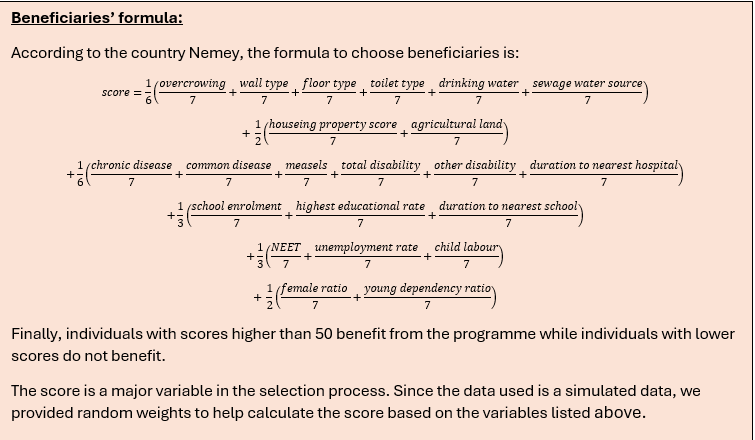
\includegraphics[keepaspectratio]{images/CH5T1.PNG}}

\begin{Shaded}
\begin{Highlighting}[]
\CommentTok{\# 2| PMT estimation }
\SpecialCharTok{{-}{-}{-}{-}{-}{-}{-}{-}{-}{-}{-}{-}{-}{-}{-}{-}{-}{-}{-}{-}{-}{-}{-}{-}{-}{-}{-}{-}{-}{-}{-}{-}{-}{-}{-}{-}{-}{-}{-}{-}{-}{-}{-}{-}{-}{-}{-}{-}{-}{-}{-}{-}{-}{-}}
\NormalTok{SCORING }\OtherTok{=}\NormalTok{ PMTIndicators }\SpecialCharTok{\%\textgreater{}\%} 
  \FunctionTok{mutate}\NormalTok{(}
    \AttributeTok{s\_var\_overcrowdingIssue =}\NormalTok{ (}\DecValTok{1}\SpecialCharTok{/}\DecValTok{6}\NormalTok{) }\SpecialCharTok{*}\NormalTok{ (}\DecValTok{1}\SpecialCharTok{/}\DecValTok{7}\NormalTok{) }\SpecialCharTok{*}\NormalTok{ var\_overcrowdingIssue, }
    \AttributeTok{s\_var\_Floor =}\NormalTok{ (}\DecValTok{1}\SpecialCharTok{/}\DecValTok{6}\NormalTok{) }\SpecialCharTok{*}\NormalTok{ (}\DecValTok{1}\SpecialCharTok{/}\DecValTok{7}\NormalTok{) }\SpecialCharTok{*}\NormalTok{ var\_Floor\_type,}
    \AttributeTok{s\_var\_Toilet =}\NormalTok{ (}\DecValTok{1}\SpecialCharTok{/}\DecValTok{6}\NormalTok{) }\SpecialCharTok{*}\NormalTok{ (}\DecValTok{1}\SpecialCharTok{/}\DecValTok{7}\NormalTok{) }\SpecialCharTok{*}\NormalTok{ var\_Toilet\_Type,}
    \AttributeTok{s\_var\_DrinkWater =}\NormalTok{ (}\DecValTok{1}\SpecialCharTok{/}\DecValTok{6}\NormalTok{) }\SpecialCharTok{*}\NormalTok{ (}\DecValTok{1}\SpecialCharTok{/}\DecValTok{7}\NormalTok{) }\SpecialCharTok{*}\NormalTok{ var\_Drinking\_water,}
    \AttributeTok{s\_var\_Sewage =}\NormalTok{ (}\DecValTok{1}\SpecialCharTok{/}\DecValTok{6}\NormalTok{) }\SpecialCharTok{*}\NormalTok{ (}\DecValTok{1}\SpecialCharTok{/}\DecValTok{7}\NormalTok{) }\SpecialCharTok{*}\NormalTok{ var\_sewage,}
    
    \AttributeTok{s\_var\_Property =}\NormalTok{ (}\DecValTok{1}\SpecialCharTok{/}\DecValTok{2}\NormalTok{) }\SpecialCharTok{*}\NormalTok{ (}\DecValTok{1}\SpecialCharTok{/}\DecValTok{7}\NormalTok{) }\SpecialCharTok{*}\NormalTok{ var\_Property\_score,}
    \AttributeTok{s\_var\_agriLand =}\NormalTok{ (}\DecValTok{1}\SpecialCharTok{/}\DecValTok{2}\NormalTok{) }\SpecialCharTok{*}\NormalTok{ (}\DecValTok{1}\SpecialCharTok{/}\DecValTok{7}\NormalTok{) }\SpecialCharTok{*}\NormalTok{ var\_AgriLand,}
    
    \AttributeTok{s\_var\_chronic =}\NormalTok{ (}\DecValTok{1}\SpecialCharTok{/}\DecValTok{6}\NormalTok{) }\SpecialCharTok{*}\NormalTok{ (}\DecValTok{1}\SpecialCharTok{/}\DecValTok{7}\NormalTok{) }\SpecialCharTok{*}\NormalTok{ var\_chronic,}
    \AttributeTok{s\_var\_common =}\NormalTok{ (}\DecValTok{1}\SpecialCharTok{/}\DecValTok{6}\NormalTok{) }\SpecialCharTok{*}\NormalTok{ (}\DecValTok{1}\SpecialCharTok{/}\DecValTok{7}\NormalTok{) }\SpecialCharTok{*}\NormalTok{ var\_common,}
    \AttributeTok{s\_var\_measels =}\NormalTok{ (}\DecValTok{1}\SpecialCharTok{/}\DecValTok{6}\NormalTok{) }\SpecialCharTok{*}\NormalTok{ (}\DecValTok{1}\SpecialCharTok{/}\DecValTok{7}\NormalTok{) }\SpecialCharTok{*}\NormalTok{ var\_measels,}
    \AttributeTok{s\_var\_totdisab =}\NormalTok{ (}\DecValTok{1}\SpecialCharTok{/}\DecValTok{6}\NormalTok{) }\SpecialCharTok{*}\NormalTok{ (}\DecValTok{1}\SpecialCharTok{/}\DecValTok{7}\NormalTok{) }\SpecialCharTok{*}\NormalTok{ var\_tot\_disab,}
    \AttributeTok{s\_var\_otherdisab =}\NormalTok{ (}\DecValTok{1}\SpecialCharTok{/}\DecValTok{6}\NormalTok{) }\SpecialCharTok{*}\NormalTok{ (}\DecValTok{1}\SpecialCharTok{/}\DecValTok{7}\NormalTok{) }\SpecialCharTok{*}\NormalTok{ var\_other\_disab,}
    \AttributeTok{s\_var\_durationHospital =}\NormalTok{ (}\DecValTok{1}\SpecialCharTok{/}\DecValTok{6}\NormalTok{) }\SpecialCharTok{*}\NormalTok{ (}\DecValTok{1}\SpecialCharTok{/}\DecValTok{7}\NormalTok{) }\SpecialCharTok{*}\NormalTok{ var\_duration\_hospital,}
    
    \AttributeTok{s\_var\_enrolment =}\NormalTok{ (}\DecValTok{1}\SpecialCharTok{/}\DecValTok{3}\NormalTok{) }\SpecialCharTok{*}\NormalTok{ (}\DecValTok{1}\SpecialCharTok{/}\DecValTok{7}\NormalTok{) }\SpecialCharTok{*}\NormalTok{ var\_enrolment,}
    \AttributeTok{s\_var\_higheducation =}\NormalTok{ (}\DecValTok{1}\SpecialCharTok{/}\DecValTok{3}\NormalTok{) }\SpecialCharTok{*}\NormalTok{ (}\DecValTok{1}\SpecialCharTok{/}\DecValTok{7}\NormalTok{) }\SpecialCharTok{*}\NormalTok{ var\_high\_education\_rate,}
    \AttributeTok{s\_var\_durationSchool =}\NormalTok{ (}\DecValTok{1}\SpecialCharTok{/}\DecValTok{3}\NormalTok{) }\SpecialCharTok{*}\NormalTok{ (}\DecValTok{1}\SpecialCharTok{/}\DecValTok{7}\NormalTok{) }\SpecialCharTok{*}\NormalTok{ var\_duration\_school,}
    
    \AttributeTok{s\_var\_NEET =}\NormalTok{ (}\DecValTok{1}\SpecialCharTok{/}\DecValTok{3}\NormalTok{) }\SpecialCharTok{*}\NormalTok{ (}\DecValTok{1}\SpecialCharTok{/}\DecValTok{7}\NormalTok{) }\SpecialCharTok{*}\NormalTok{ var\_NEET,}
    \AttributeTok{s\_var\_unemp =}\NormalTok{ (}\DecValTok{1}\SpecialCharTok{/}\DecValTok{3}\NormalTok{) }\SpecialCharTok{*}\NormalTok{ (}\DecValTok{1}\SpecialCharTok{/}\DecValTok{7}\NormalTok{) }\SpecialCharTok{*}\NormalTok{ var\_unemployment\_rate,}
    \AttributeTok{s\_var\_childLabour =}\NormalTok{ (}\DecValTok{1}\SpecialCharTok{/}\DecValTok{3}\NormalTok{) }\SpecialCharTok{*}\NormalTok{ (}\DecValTok{1}\SpecialCharTok{/}\DecValTok{7}\NormalTok{) }\SpecialCharTok{*}\NormalTok{ var\_child\_labour,}
    
    \AttributeTok{s\_var\_female =}\NormalTok{ (}\DecValTok{1}\SpecialCharTok{/}\DecValTok{2}\NormalTok{) }\SpecialCharTok{*}\NormalTok{ (}\DecValTok{1}\SpecialCharTok{/}\DecValTok{7}\NormalTok{) }\SpecialCharTok{*}\NormalTok{ var\_female\_ratio,}
    \AttributeTok{s\_var\_youngdependency =}\NormalTok{ (}\DecValTok{1}\SpecialCharTok{/}\DecValTok{2}\NormalTok{) }\SpecialCharTok{*}\NormalTok{ (}\DecValTok{1}\SpecialCharTok{/}\DecValTok{7}\NormalTok{) }\SpecialCharTok{*}\NormalTok{ var\_young\_dependency\_ratio,}
    
    \AttributeTok{score =}\NormalTok{ s\_var\_overcrowdingIssue }\SpecialCharTok{+}\NormalTok{ s\_var\_Wall }\SpecialCharTok{+}\NormalTok{ s\_var\_Floor }\SpecialCharTok{+}\NormalTok{ s\_var\_Toilet }\SpecialCharTok{+}\NormalTok{ s\_var\_DrinkWater }\SpecialCharTok{+}\NormalTok{ s\_var\_Sewage }\SpecialCharTok{+}
\NormalTok{      s\_var\_Property }\SpecialCharTok{+}\NormalTok{ s\_var\_agriLand }\SpecialCharTok{+}\NormalTok{ s\_var\_chronic }\SpecialCharTok{+}\NormalTok{ s\_var\_common }\SpecialCharTok{+}\NormalTok{ s\_var\_measels }\SpecialCharTok{+}\NormalTok{ s\_var\_totdisab }\SpecialCharTok{+}\NormalTok{ s\_var\_otherdisab }\SpecialCharTok{+}
\NormalTok{      s\_var\_durationHospital }\SpecialCharTok{+}\NormalTok{ s\_var\_enrolment }\SpecialCharTok{+}\NormalTok{ s\_var\_higheducation }\SpecialCharTok{+}\NormalTok{ s\_var\_durationSchool }\SpecialCharTok{+}\NormalTok{ s\_var\_NEET }\SpecialCharTok{+}\NormalTok{ s\_var\_unemp }\SpecialCharTok{+}
\NormalTok{      s\_var\_childLabour }\SpecialCharTok{+}\NormalTok{ s\_var\_female }\SpecialCharTok{+}\NormalTok{ s\_var\_youngdependency}
\NormalTok{  ) }\SpecialCharTok{\%\textgreater{}\%}
  \FunctionTok{drop\_na}\NormalTok{()}
\end{Highlighting}
\end{Shaded}

\subsection{\texorpdfstring{\textbf{3.
Clustering}}{3. Clustering}}\label{clustering}

This section explains the conceptual elements of statistical clustering.
While it introduces the basic concepts, it primarily focuses on the
clustering methods recommended for the SPP-RAF. For those interested in
a deeper exploration, Zelterman (2015) \footnote{Zelterman, D. (2015).
  \emph{Applied Multivariate Statisticas with R.} New Haven: Springer.}
provides an excellent resource, particularly Chapters 11 and 10 (in that
order).

The problem of clustering is relatively easy to state: given a set of
individuals with different traits, the goal is to group them into
clusters where the characteristics within each group are similar, and
the characteristics between groups are distinct. However, this seemingly
simple definition raises two key challenges:

\begin{enumerate}
\def\labelenumi{\arabic{enumi}.}
\tightlist
\item
  What criteria should be used to define similarity or dissimilarity
  between two individuals (Step 1)?
\item
  How can we determine when two individuals are too different to belong
  to the same group (Step 2)?
\end{enumerate}

Each of these questions presents multiple alternatives and
methodological challenges. As with previous topics, there is no single
correct answer. Indeed, the ``Ugly Duckling'' theorem\footnote{Watanabe,
  S. (1969). \emph{Knowing and guessing; a quantitative study of
  inference and information.} New York: Wiley.} demonstrates that
clustering always involves a degree of subjectivity. Consequently,
analysts must rely on their domain knowledge to interpret data
effectively within the given context.

\subsubsection{Step 1: Distances}\label{step-1-distances}

The first step in clustering is defining a measure of distance between
individuals. Several distance metrics can be used, each with different
properties and implications. Among the most common is the Euclidean
metric, which measures the straight-line distance between two points
\(p\) and \(q\), computed using the Pythagorean Theorem.

\paragraph{Example}\label{example}

Ahmed is 40 years old with 20 years of work experience, whereas Mohammed
is 37.5 years old with 15 years of experience. The Euclidean distance
between them is: \[ \sqrt{(40 - 37.5)^2 + (20 - 15)^2} = 5.59 \]

Other distance metrics include: \textbf{Manhattan distance}, which is
more robust to outliers because it does not square differences.
\textbf{Jaccard index}, which measures similarity between categorical
data. The Jaccard distance is derived by subtracting the index value
from 1.

\paragraph{Scale Considerations}\label{scale-considerations}

One crucial aspect when working with distances is the scale of the
observations. Consider the following individuals: - Ahmed: 40 years old,
20 years of work experience - Mona: 40 years old, 15 years of work
experience - Maryam: 37.5 years old, 20 years of work experience -
Mohammed: 37.5 years old, 15 years of work experience

Using the Euclidean metric, the distance between Maryam and Mona is also
5.59, the same as between Ahmed and Mohammed. However, if we measure age
in days instead of years, the distances become 16,303 for the men and
15,572 for the women. This shift alters the ratio between the two
distances (previously 1, now 1.05), affecting the clustering outcome.
Thus, proper standardization or transformation of variables is necessary
to maintain consistency.

Another issue arises from the relationship between age and work
experience. As shown in Figure 3.1, these variables are highly
correlated. While geometrically the four individuals appear equidistant,
conceptually they are not. Ahmed and Mohammed follow a common pattern,
whereas Maryam and Mona deviate from it. Proper adjustments using
covariance transformations can address this issue.

\emph{Figure 3.1 Example of age vs working experience}

\pandocbounded{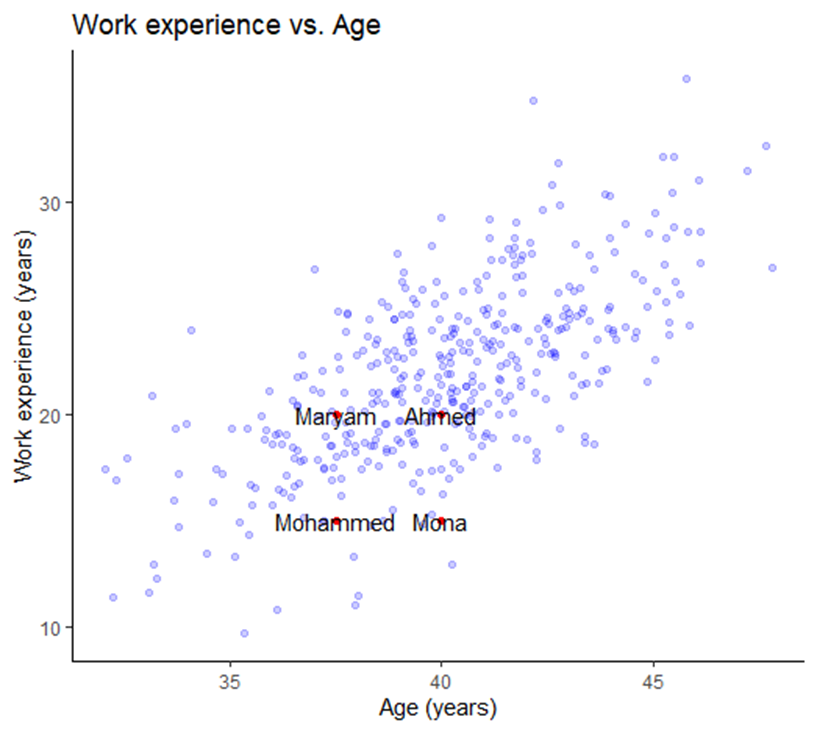
\includegraphics[keepaspectratio]{images/clipboard-461174848.png}}

\paragraph{Mahalanobis Distance}\label{mahalanobis-distance}

A more sophisticated alternative to Euclidean distance is the
\textbf{Mahalanobis distance}\footnote{Mahalanobis, P. C. (1936). On the
  generalized distance in statistics. \emph{Proceedings of the National
  Institute of Sciences of India}, 49-55.}, which accounts for
correlations among variables. This metric is invariant to scale and
incorporates covariance structures, making it particularly useful for
clustering multivariate data. The later sections explain how to
implement Mahalanobis distance in R.

Additionally, when assessing distances between multivariate datasets, it
is useful to consider not just the direct distance between two points
but also their distance relative to a distribution. The Mahalanobis
metric achieves this by incorporating the inverse covariance matrix,
making it effective for imbalanced datasets and one-class
classification.

\subsubsection{Step 2: Clustering}\label{step-2-clustering}

The clustering method proposed here is \textbf{hierarchical clustering},
using a bottom-up approach. The code implements hierarchical clustering
with \textbf{Ward linkage}, which minimizes variance within clusters,
leading to balanced groupings.

Other linkage methods include \textbf{Single linkage (nearest neighbor
linkage):} Useful for identifying irregularly shaped clusters, and
\textbf{Complete linkage (farthest neighbor linkage):} Produces more
compact clusters.

These methods are not implemented in the provided code but could be
useful depending on the dataset.

There is no universal guideline for selecting a clustering method; it is
recommended to test different linkages to determine which best reflects
the data. However, Ward linkage is often preferred when the goal is to
obtain balanced clusters, as other methods may produce highly unbalanced
structures.

Once a decision tree is generated, the next challenge at the policy
level is determining the number of clusters required for profiling. For
instance, if policymakers aim to create three distinct targeting
strategies, the corresponding dendrogram can help determine the
appropriate cut-off.

\subsubsection{Step 3: Classification}\label{step-3-classification}

While clustering helps group individuals, it does not explain why
individuals are classified in a particular way. To address this, two
techniques are used: 1. A descriptive approach (explained via examples).
2. A technical approach using \textbf{classification and regression
trees (CART)}\footnote{Breiman, L. (1984). Classification and regression
  trees. \emph{The Wadsworth and Brooks-Cole statisticsprobability
  series.} Chapman \& Hall.}, a fundamental technique in machine
learning.

\paragraph{Example}\label{example-1}

A target variable has four classes represented by different colors:
Yellow (4 observations), Orange (5 observations), Green (8
observations), and Blue (10 observations).

The largest group is blue, so if no further information is available,
the default classification is blue. However, by incorporating additional
variables---such as work experience, the algorithm refines the
classification. If an individual has over 25 years of experience, they
are assigned to the orange category. Further refinements occur with
additional splits.

While it is possible to continue dividing the tree until each node
contains only one class, this leads to \textbf{overfitting}, where the
model captures noise rather than meaningful patterns. Overfitting can
result in misclassifications caused by minor data inconsistencies (e.g.,
typographical errors). Therefore, the balance between accuracy and
generalization must be considered. For avid readers, the book of Gareth
et al.~(2017)\footnote{Gareth, J., Witten, D., Hastie, T., \&
  Tibshirani, R. (2017). \emph{An Introduction to Statistical Learning:
  with Applications in R.} New York: Springer.} provides an in-depth
analysis of this issue. However for the readers interested in the
concept but not in the details, the following link provides practical
explanations about the
\href{https://towardsdatascience.com/how-to-find-decision-tree-depth-via-cross-validation-2bf143f0f3d6.}{decision
tree depth}

While the manual does not provide a line-by-line walkthrough of the
code, the complete implementation is included. The code is thoroughly
commented to explain the logic and facilitate understanding, allowing
readers to follow the methodology and adapt it as needed.

\subsubsection{Custom implementation for clustering
(optional)}\label{custom-implementation-for-clustering-optional}

This section introduces the R code used for clustering (identified
Manual Final/Code/Aux - Functions.R). In previous methods, the number of
clusters was determined automatically, often resulting in groups with
minimal observations. In contrast, the new approach specifies both the
number of cuts and the final number of clusters to ensure meaningful
segmentation.

The provided R code is a custom implementation for clustering and
decision tree generation. Unlike traditional packages, this approach: -
Handles both numeric and categorical data. - Includes a custom metric
(\texttt{findingX}) to optimize cluster splits. - Ensures a minimum
cluster size (\texttt{basketLimit}). - Uses squared Euclidean distance
for robustness. - Incorporates decision trees (\texttt{rpart}) for
classification.

Three key functions are used: 1. \textbf{\texttt{findingX}}: Identifies
optimal cut points for clustering. 2. \textbf{\texttt{treeGraph}}:
Generates a network visualization of clusters. 3.
\textbf{\texttt{clusteringFunction}}: Executes clustering, refines
clusters, and builds a decision tree.

This custom framework enables clustering across \textbf{46 variables for
150 observations}, specifically for Governorate A. The \textbf{distance
matrix applies to PMT variables}, but clusters are profiled based on
additional attributes (e.g., gender, region).

Despite its advantages, this method is computationally intensive. Users
seeking a simpler approach may consider standard algorithms such as
\texttt{kmeans} or \texttt{hclust}. However, this tailored approach
ensures policy-relevant constraints and maintains cluster
interpretability.

For the purpose of the code, we assume that the government of Nemey is
interested in 5 groups or cluster, meaning that Nemey would like to
categorize at least 5 types of beneficiaries. At the beginning of the
code there are some commands to prepare the datasets according to PMT
and scoring estimated previously.

\begin{Shaded}
\begin{Highlighting}[]
\NormalTok{ basketLimit}\OtherTok{=}\FunctionTok{max}\NormalTok{(}\DecValTok{15}\NormalTok{,}\FunctionTok{ceiling}\NormalTok{(}\FunctionTok{dim}\NormalTok{(BeneficiariesData)[}\DecValTok{1}\NormalTok{]}\SpecialCharTok{*}\FloatTok{0.025}\NormalTok{)) }
\NormalTok{ PolicyGroups}\OtherTok{=}\DecValTok{5} 
 \FunctionTok{source}\NormalTok{() }\CommentTok{\#Clustering Function\textquotesingle{}results are saved in  result List }
\NormalTok{ resultList}\OtherTok{=}\FunctionTok{clusteringFunction}\NormalTok{(BeneficiariesSelectionData, BeneficiariesDistanceData, basketLimit, PolicyGroups)}
\end{Highlighting}
\end{Shaded}

After the custom version of the clustering is executed, it is suggested
to use decision trees which serve as both a refinement tool and an
explanation mechanism for the clustering results.

In the code the first stage builds a constrained-depth decision tree
(max depth = 4) to establish broad cluster definitions, while the second
stage creates a more granular tree (minimum 2 observations per node) to
capture finer patterns. By using extremely small complexity parameters
(cp ≈ 0), the algorithm prioritizes capturing the true cluster structure
over preventing overfitting. The final output includes both a visual
decision tree (via \texttt{rpart.plot}) which explains cluster
membership rules in terms of the original variables, and a frequency
table summarizing the distribution of refined clusters. This approach is
particularly valuable for gaining a deeper understanding of beneficiary
characteristics.

\subsubsection{Step 4. Descriptive statistics to assess the
clusters}\label{step-4.-descriptive-statistics-to-assess-the-clusters}

It is recommended to create a report, with visualizations and summary
tables of results from the clustering analysis exercise. The script, on
the section 3.5 and owndars, contains a section that creats a workbook
and then adds three main sections: (1) a dendrogram showing how data
points are grouped into clusters (Figure 3.2), (2) a decision tree
explaining the clustering rules , and (3) descriptive graphs comparing
cluster characteristics/bar charts for categorical variables and average
values for numerical variables. Each section includes formatted plots
(saved as PNGs) alongside supporting data tables, with text dynamically
adjusted for either English or Arabic based on a language flag.

The code automates the entire reporting workflow---from generating plots
with consistent styling (fonts, colors, labels) to organizing them in
Excel with proper spacing. It manages scaling, positioning, and
language-specific formatting, then produces two final versions of the
report: one in English (\texttt{CH\ 1\ EN.xlsx}) and one in Arabic
(\texttt{CH\ 1\ AR.xlsx}). The result is a polished, ready-to-share
analysis that explains how clusters were formed and what differentiates
them. Below you can find a chunk creating the wb workbook and parameters
for the Excel sheet that will save the dendogram in the Figure 3.2
(language AR).

\begin{Shaded}
\begin{Highlighting}[]

\CommentTok{\# 3.5| Graphs}
\NormalTok{wb }\OtherTok{=}\NormalTok{ openxlsx}\SpecialCharTok{::}\FunctionTok{createWorkbook}\NormalTok{(}\AttributeTok{creator =} \StringTok{\textquotesingle{}ESCWA\textquotesingle{}}\NormalTok{)}

\CommentTok{\# 3.5.1| Dendrogram }
\NormalTok{rowLine }\OtherTok{=} \DecValTok{1}
\NormalTok{jumpOfRows }\OtherTok{=} \DecValTok{18}
\NormalTok{colPlots }\OtherTok{=} \DecValTok{1}
\NormalTok{colTables }\OtherTok{=} \DecValTok{12}

\CommentTok{\# Specify an indicatorCOde to be used as the name of the graph}
\NormalTok{indicatorCode }\OtherTok{\textless{}{-}} \StringTok{\textquotesingle{}1\_0\textquotesingle{}}
\NormalTok{part }\OtherTok{\textless{}{-}} \StringTok{\textquotesingle{}\textquotesingle{}}
\NormalTok{labCodes }\OtherTok{\textless{}{-}}\NormalTok{ dataPlots }\SpecialCharTok{\%\textgreater{}\%} \FunctionTok{subset}\NormalTok{(Code }\SpecialCharTok{==} \FunctionTok{paste0}\NormalTok{(indicatorCode, part))}
\NormalTok{newSheet }\OtherTok{\textless{}{-}} \FunctionTok{addWorksheet}\NormalTok{(wb, }\AttributeTok{sheetName =}\NormalTok{ indicatorCode)}


\CommentTok{\# To export:}
\NormalTok{base\_exp }\OtherTok{=} \DecValTok{1}
\NormalTok{heightExp }\OtherTok{=} \FloatTok{1.5}
\NormalTok{widthExp }\OtherTok{=} \FloatTok{1.2}
\NormalTok{scale\_factor }\OtherTok{=}\NormalTok{ base\_exp}\SpecialCharTok{/}\NormalTok{widthExp}

\CommentTok{\# Cut same as number of maximum clusters}
\NormalTok{cutNumber}\OtherTok{=}\NormalTok{PolicyGroups}
\NormalTok{newPlot }\OtherTok{=} \FunctionTok{fviz\_dend}\NormalTok{(clust, }\AttributeTok{k =}\NormalTok{ cutNumber, }\AttributeTok{color\_labels\_by\_k =}\NormalTok{ T, }\AttributeTok{palette =} \FunctionTok{as.character}\NormalTok{(labCodes[, }\DecValTok{12}\NormalTok{]), }\AttributeTok{show\_labels =}\NormalTok{ F,}
                    \AttributeTok{rect =}\NormalTok{ T, }\AttributeTok{lower\_rect =} \SpecialCharTok{{-}}\FloatTok{0.02}\NormalTok{, }\AttributeTok{rect\_border =} \FunctionTok{as.character}\NormalTok{(labCodes[, }\DecValTok{12}\NormalTok{]), }\AttributeTok{rect\_fill =}\NormalTok{ T) }\SpecialCharTok{+}
  \FunctionTok{labs}\NormalTok{(}\AttributeTok{title =} \FunctionTok{paste0}\NormalTok{(}\FunctionTok{as.character}\NormalTok{(labCodes[, }\DecValTok{5}\SpecialCharTok{*}\NormalTok{(}\DecValTok{1}\SpecialCharTok{{-}}\NormalTok{language)}\SpecialCharTok{+}\DecValTok{2}\NormalTok{])),}
       \AttributeTok{subtitle =} \FunctionTok{as.character}\NormalTok{(labCodes[, }\DecValTok{5}\SpecialCharTok{*}\NormalTok{(}\DecValTok{1}\SpecialCharTok{{-}}\NormalTok{language)}\SpecialCharTok{+}\DecValTok{3}\NormalTok{]),}
       \AttributeTok{caption =} \FunctionTok{as.character}\NormalTok{(labCodes[, }\DecValTok{5}\SpecialCharTok{*}\NormalTok{(}\DecValTok{1}\SpecialCharTok{{-}}\NormalTok{language)}\SpecialCharTok{+}\DecValTok{6}\NormalTok{]),}
       \AttributeTok{x =} \FunctionTok{as.character}\NormalTok{(labCodes[, }\DecValTok{5}\SpecialCharTok{*}\NormalTok{(}\DecValTok{1}\SpecialCharTok{{-}}\NormalTok{language)}\SpecialCharTok{+}\DecValTok{4}\NormalTok{]),}
       \AttributeTok{y =} \FunctionTok{as.character}\NormalTok{(labCodes[, }\DecValTok{5}\SpecialCharTok{*}\NormalTok{(}\DecValTok{1}\SpecialCharTok{{-}}\NormalTok{language)}\SpecialCharTok{+}\DecValTok{5}\NormalTok{])) }\SpecialCharTok{+}
  \FunctionTok{scale\_y\_continuous}\NormalTok{(}\AttributeTok{position =} \ControlFlowTok{if}\NormalTok{ (language }\SpecialCharTok{==} \DecValTok{0}\NormalTok{) \{}\StringTok{\textquotesingle{}right\textquotesingle{}}\NormalTok{\} }\ControlFlowTok{else}\NormalTok{ \{}\StringTok{\textquotesingle{}left\textquotesingle{}}\NormalTok{\}) }\SpecialCharTok{+} 
  \FunctionTok{theme\_classic}\NormalTok{() }\SpecialCharTok{+}
  \FunctionTok{theme}\NormalTok{(}\AttributeTok{legend.position =} \StringTok{\textquotesingle{}bottom\textquotesingle{}}\NormalTok{,}
        \AttributeTok{text =} \FunctionTok{element\_text}\NormalTok{(}\AttributeTok{family =} \StringTok{\textquotesingle{}Georgia\textquotesingle{}}\NormalTok{),}
        \AttributeTok{axis.line.x =} \FunctionTok{element\_blank}\NormalTok{(),}
        \AttributeTok{axis.line.y =} \FunctionTok{element\_blank}\NormalTok{(),}
        \AttributeTok{axis.text.x =} \FunctionTok{element\_blank}\NormalTok{(),}
        \AttributeTok{axis.ticks.x =} \FunctionTok{element\_blank}\NormalTok{(),}
        \AttributeTok{axis.text.y =} \FunctionTok{element\_text}\NormalTok{(}\AttributeTok{size =}\NormalTok{ scale\_factor }\SpecialCharTok{*} \DecValTok{10}\NormalTok{, }\AttributeTok{family =} \StringTok{\textquotesingle{}Georgia\textquotesingle{}}\NormalTok{),}
        \AttributeTok{axis.title.x =} \FunctionTok{element\_text}\NormalTok{(}\AttributeTok{hjust =} \FloatTok{0.5}\NormalTok{, }\AttributeTok{size =}\NormalTok{ scale\_factor }\SpecialCharTok{*} \DecValTok{10}\NormalTok{, }\AttributeTok{family =} \StringTok{\textquotesingle{}Georgia\textquotesingle{}}\NormalTok{),}
        \AttributeTok{axis.title.y =} \FunctionTok{element\_text}\NormalTok{(}\AttributeTok{hjust =} \FloatTok{0.5}\NormalTok{, }\AttributeTok{size =}\NormalTok{ scale\_factor }\SpecialCharTok{*} \DecValTok{10}\NormalTok{, }\AttributeTok{family =} \StringTok{\textquotesingle{}Georgia\textquotesingle{}}\NormalTok{),}
        \AttributeTok{legend.text =} \FunctionTok{element\_text}\NormalTok{(}\AttributeTok{size =}\NormalTok{ scale\_factor }\SpecialCharTok{*} \DecValTok{10}\NormalTok{, }\AttributeTok{family =} \StringTok{\textquotesingle{}Georgia\textquotesingle{}}\NormalTok{),}
        \AttributeTok{strip.text =} \FunctionTok{element\_text}\NormalTok{(}\AttributeTok{size =}\NormalTok{ scale\_factor }\SpecialCharTok{*} \DecValTok{10}\NormalTok{, }\AttributeTok{family =} \StringTok{\textquotesingle{}Georgia\textquotesingle{}}\NormalTok{),}
        \AttributeTok{plot.title =} \FunctionTok{element\_text}\NormalTok{(}\AttributeTok{face =} \StringTok{\textquotesingle{}bold\textquotesingle{}}\NormalTok{, }\AttributeTok{size =} \DecValTok{10}\NormalTok{, }\AttributeTok{family =} \StringTok{\textquotesingle{}Georgia\textquotesingle{}}\NormalTok{, }\AttributeTok{hjust =} \ControlFlowTok{if}\NormalTok{ (language }\SpecialCharTok{==} \DecValTok{0}\NormalTok{) \{}\DecValTok{1}\NormalTok{\} }\ControlFlowTok{else}\NormalTok{ \{}\DecValTok{0}\NormalTok{\}),}
        \AttributeTok{plot.subtitle =} \FunctionTok{element\_text}\NormalTok{(}\AttributeTok{size =} \DecValTok{10}\NormalTok{, }\AttributeTok{family =} \StringTok{\textquotesingle{}Georgia\textquotesingle{}}\NormalTok{, }\AttributeTok{hjust =} \ControlFlowTok{if}\NormalTok{ (language }\SpecialCharTok{==} \DecValTok{0}\NormalTok{) \{}\DecValTok{1}\NormalTok{\} }\ControlFlowTok{else}\NormalTok{ \{}\DecValTok{0}\NormalTok{\}),}
        \AttributeTok{legend.key.size =} \FunctionTok{unit}\NormalTok{(}\FloatTok{0.5} \SpecialCharTok{*}\NormalTok{ scale\_factor, }\StringTok{\textquotesingle{}cm\textquotesingle{}}\NormalTok{))}

\CommentTok{\# Export graph and table to excel:}
\NormalTok{fileName }\OtherTok{=} \FunctionTok{paste0}\NormalTok{(}\AttributeTok{fileName =} \FunctionTok{paste0}\NormalTok{(outputLocation, indicatorCode, part, }
                                    \ControlFlowTok{if}\NormalTok{(language }\SpecialCharTok{==} \DecValTok{1}\NormalTok{) \{}\StringTok{\textquotesingle{} (English)\textquotesingle{}}\NormalTok{\} }\ControlFlowTok{else}\NormalTok{ \{}\StringTok{\textquotesingle{} (Arab)\textquotesingle{}}\NormalTok{\}, }\StringTok{\textquotesingle{}.png\textquotesingle{}}\NormalTok{))}

\FunctionTok{ggsave}\NormalTok{(fileName, }\AttributeTok{plot =}\NormalTok{ newPlot, }\AttributeTok{width =} \DecValTok{6} \SpecialCharTok{*}\NormalTok{ widthExp, }\AttributeTok{height =} \DecValTok{4} \SpecialCharTok{*}\NormalTok{ heightExp }\SpecialCharTok{*}\NormalTok{ widthExp, }\AttributeTok{scale =}\NormalTok{ scale\_factor)}
\FunctionTok{insertImage}\NormalTok{(wb, }\AttributeTok{file =}\NormalTok{ fileName, }\AttributeTok{sheet =}\NormalTok{ indicatorCode, }\AttributeTok{startRow =}\NormalTok{ rowLine, }\AttributeTok{startCol =}\NormalTok{ colPlots, }\AttributeTok{width =} \DecValTok{6} \SpecialCharTok{*}\NormalTok{ widthExp, }\AttributeTok{height =} \DecValTok{4} \SpecialCharTok{*}\NormalTok{ heightExp }\SpecialCharTok{*}\NormalTok{ widthExp)}

\NormalTok{newData}\OtherTok{=}\FunctionTok{as.data.frame}\NormalTok{(}\FunctionTok{as.matrix}\NormalTok{(}\FunctionTok{table}\NormalTok{(resultList}\SpecialCharTok{$}\NormalTok{aggregatedCluster)))}\SpecialCharTok{\%\textgreater{}\%}
  \FunctionTok{mutate}\NormalTok{(}\AttributeTok{Clusters=}\FunctionTok{rownames}\NormalTok{(}\FunctionTok{table}\NormalTok{(resultList}\SpecialCharTok{$}\NormalTok{aggregatedCluster)))}\SpecialCharTok{\%\textgreater{}\%}
  \FunctionTok{rename}\NormalTok{(}\AttributeTok{Observations=}\NormalTok{V1)}\SpecialCharTok{\%\textgreater{}\%}
\NormalTok{  dplyr}\SpecialCharTok{::}\FunctionTok{select}\NormalTok{(Clusters,Observations)}

\FunctionTok{writeDataTable}\NormalTok{(wb, }\AttributeTok{sheet =}\NormalTok{ indicatorCode, }\AttributeTok{x =}\NormalTok{ newData, }\AttributeTok{startRow =}\NormalTok{ rowLine, }\AttributeTok{startCol =}\NormalTok{ colTables)}
\NormalTok{rowLine }\OtherTok{=}\NormalTok{ rowLine }\SpecialCharTok{+}\NormalTok{ jumpOfRows}
\end{Highlighting}
\end{Shaded}

\emph{Figure 3.2 Report of dendogram (language Arabic)}

\pandocbounded{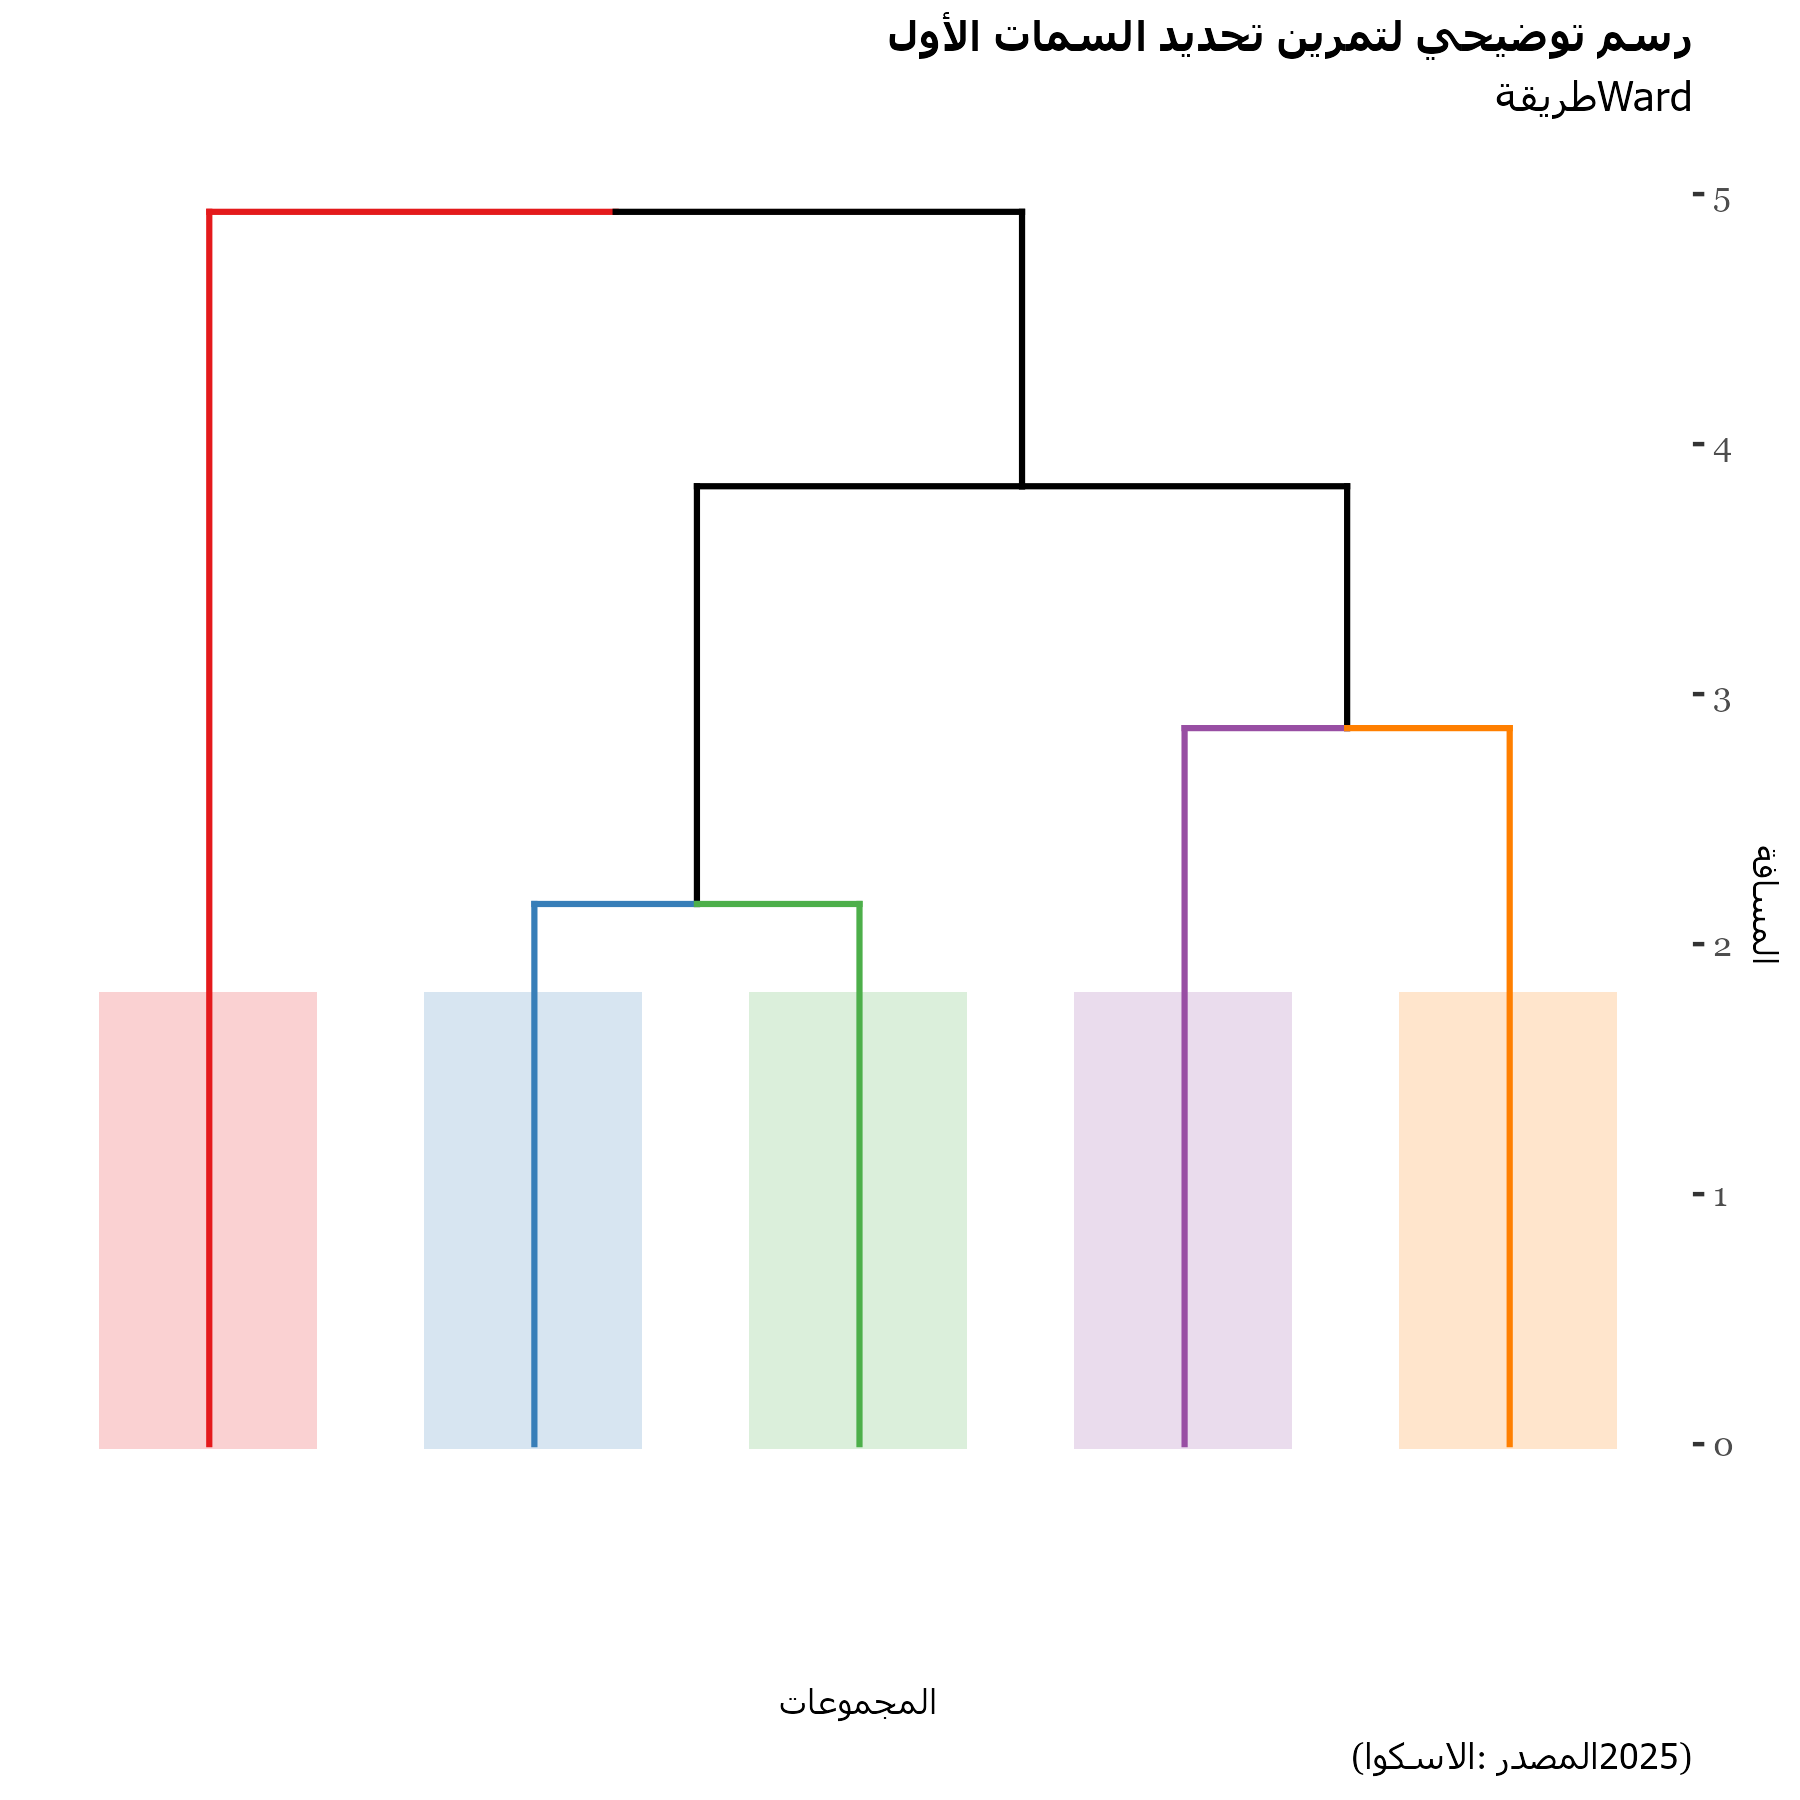
\includegraphics[keepaspectratio]{images/clipboard-3644054058.png}}\textbf{Descriptive
statistics}

To get descriptive statistics is important to distinguish between
qualitative and quantitative variables. For qualitative variables ones a
bar plot with the share by category and by cluster will be plotted while
for qualitative variables the cluster will describe the mean by
variable. To understand the type of graphs and options refer to the
Introduction R Manual. The corresponding graphs can also be found in the
Code Markdown.

\begin{Shaded}
\begin{Highlighting}[]
\CommentTok{\# Distinguishing qualitative and quantitative vars for plotting and reporting}

\NormalTok{split }\OtherTok{\textless{}{-}} \FunctionTok{splitmix}\NormalTok{(mainData) }
\FunctionTok{colnames}\NormalTok{(split}\SpecialCharTok{$}\NormalTok{X.quali)}\OtherTok{=}\FunctionTok{gsub}\NormalTok{(}\StringTok{"}\SpecialCharTok{\textbackslash{}\textbackslash{}}\StringTok{."}\NormalTok{, }\StringTok{" "}\NormalTok{, }\FunctionTok{colnames}\NormalTok{(split}\SpecialCharTok{$}\NormalTok{X.quali))}
\FunctionTok{colnames}\NormalTok{(split}\SpecialCharTok{$}\NormalTok{X.quanti)}\OtherTok{=}\FunctionTok{gsub}\NormalTok{(}\StringTok{"}\SpecialCharTok{\textbackslash{}\textbackslash{}}\StringTok{."}\NormalTok{, }\StringTok{" "}\NormalTok{, }\FunctionTok{colnames}\NormalTok{(split}\SpecialCharTok{$}\NormalTok{X.quanti))}

\NormalTok{qualiMainData}\OtherTok{=}\NormalTok{mainData}\SpecialCharTok{\%\textgreater{}\%}\NormalTok{ dplyr}\SpecialCharTok{::}\FunctionTok{select}\NormalTok{(}\FunctionTok{colnames}\NormalTok{(split}\SpecialCharTok{$}\NormalTok{X.quali))}\SpecialCharTok{\%\textgreater{}\%}
  \FunctionTok{mutate}\NormalTok{(}\AttributeTok{Clusters=}\FunctionTok{factor}\NormalTok{(originalData}\SpecialCharTok{$}\NormalTok{Clusters))}

\NormalTok{quantiMainData}\OtherTok{=}\NormalTok{mainData}\SpecialCharTok{\%\textgreater{}\%}\NormalTok{ dplyr}\SpecialCharTok{::}\FunctionTok{select}\NormalTok{(}\FunctionTok{colnames}\NormalTok{(split}\SpecialCharTok{$}\NormalTok{X.quanti))}\SpecialCharTok{\%\textgreater{}\%}
  \FunctionTok{mutate}\NormalTok{(}\AttributeTok{Clusters=}\FunctionTok{factor}\NormalTok{(originalData}\SpecialCharTok{$}\NormalTok{Clusters))}
\end{Highlighting}
\end{Shaded}

\emph{Figure 3.3 Example of descriptive statistics by cluster and
schooling level (language English)}

\pandocbounded{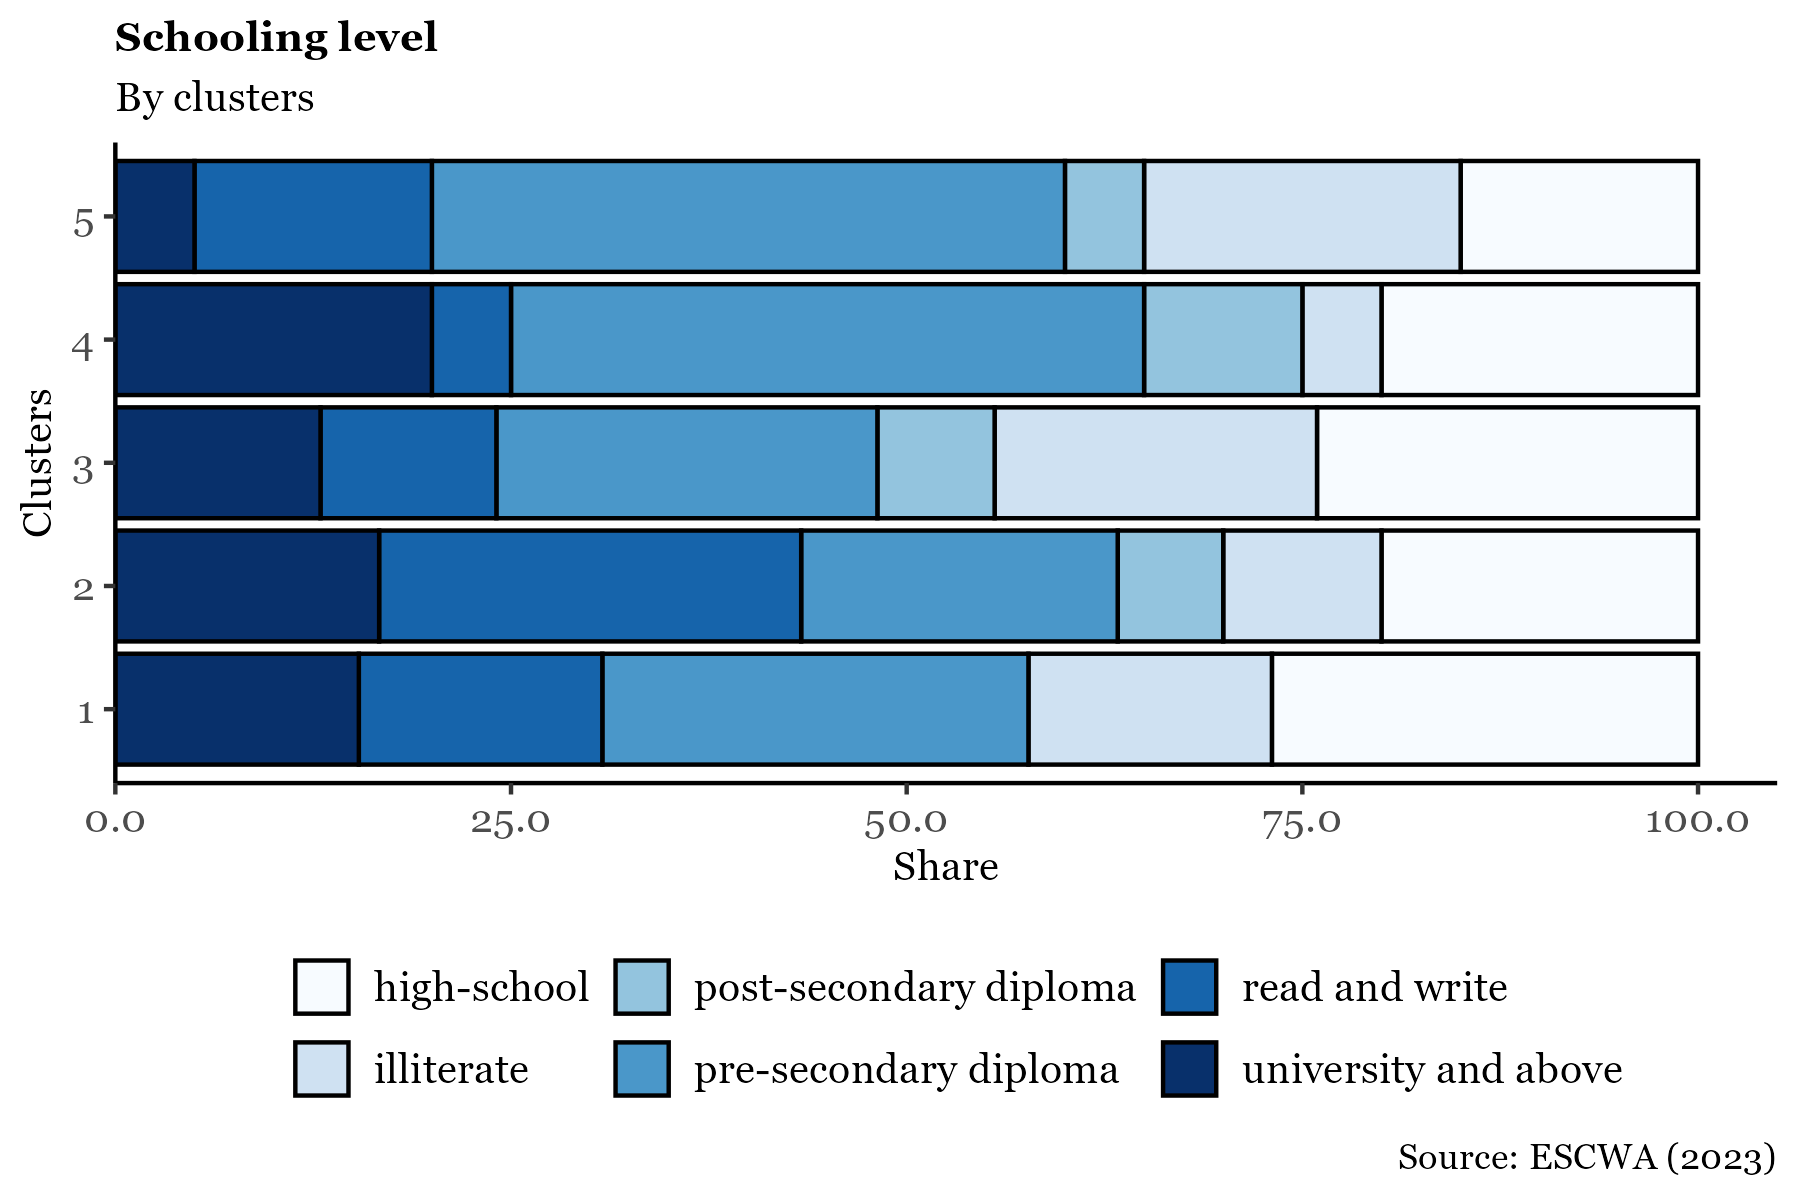
\includegraphics[keepaspectratio]{images/Prof3.png}}

For a clear visual inspection of the outputs, a heatmap highlighting the
maximum and minimum mean and proportions (for categorical variables)
could be helpful to select the main characteristics considering the
context and the purpose. In the related code there is a section
dedicated to the Cluster heatmap report. It is important not to focus on
the specific numerical values, but rather to use the table as a way to
understand the general characteristics of the households within each
cluster. The clustering applied here is based on variables used in the
PMT (Proxy Means Test) formula and those provided in the original
datasets. Although asset-related variables were indexed during
clustering to reduce co-variability, they still play a significant role
in the final results. To gain deeper analytical insights into the
differences between clusters, we recommend focusing on variables having
as suffix ``issue'' or ``rate''. Definitions of these variables could be
read in the script.

Guided by the color-coded heatmap and the selected variables shown in
the screenshot below (which you can reproduce) you can begin your own
analysis (Figure 3.4). For instance, examining gender participation
reveals that Cluster 5 is predominantly female, whereas Cluster 4 has
lower female participation and limited representation. Cluster 4 also
exhibits higher levels of urban residency and is largely composed of
single or divorced individuals, suggesting a profile of urban males who
are typically unmarried. This report will be processed automatically and
saved in the folder \emph{Output/Clustering.}

\emph{Figure 3.4 Heatmap sheet to identify cluster's characteristics}

\pandocbounded{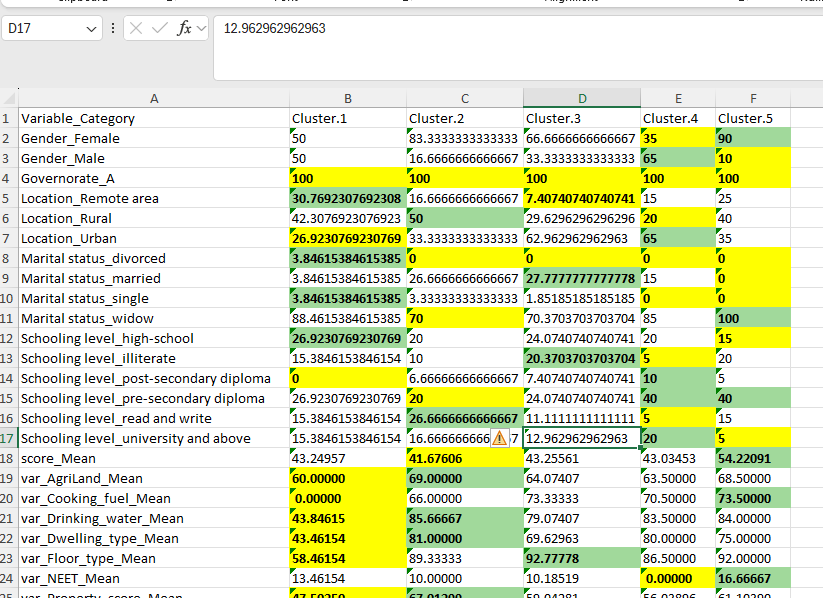
\includegraphics[keepaspectratio]{images/clipboard-2282225298.png}}

\subsection{4. Targeting assessment}\label{targeting-assessment}

Social assistance programmes have limited resources and with very few
exceptional cases, the number of resources is less than the population
that needs the support. For this reason, governments need to develop
selection criteria to choose only those that will benefit the most from
the programme. However, one thing is the conceptual design of the
strategy and another thing is its realization. For example, consider a
programme that requires people to have a mobile phone and in the region
everyone has one. Then, there isn't really a prioritization going on. Or
on the other hand, consider a programme that gives equal weight to
families with kids, and families with members that go to primary school.
As these variables are highly related, the common topic (kids in
schools) might be weighted more than other variables that can also be
relevant for choosing beneficiaries. For this reason, this chapter
develops two complementary techniques to understand how relevant the
current decision criteria for the selection of beneficiaries are.

Once the profiling of beneficiaries is completed, the next step in the
SPP-RAF framework is to evaluate the criteria used to determine
programme participation. This stage focuses on assessing the relevance
of the selection variables in relation to the beneficiary profiles
identified in the previous stage. During this phase, the scores assigned
to beneficiaries for each selection criterion are analyzed to understand
their influence on the overall eligibility score and the resulting
selection or exclusion of applicants. In this stage, the data
requirements include all variables used in the selection criteria for
beneficiaries, and the weights applied to each variable in the scoring
process.

\textbf{Outputs}:

\begin{itemize}
\item
  A set of measurements ranking the selected variables based on their
  relevance to current beneficiaries and their impact on eligibility
  scores.
\item
  A comparative analysis between filter weights and variable scores to
  assess the alignment between intended and actual beneficiaries.
\end{itemize}

\subsubsection{Variance decomposition
technique}\label{variance-decomposition-technique}

While ideally, policymakers specify the weight of each variable in the
decision criteria, in practice, once theory meets data, no strict
ordering or weighting may be evident. Consider a scenario where two
variables,~X~and~Y, are used to compute a score that determines whether
an individual qualifies for a programme. To simplify, the formula is:

\[
score= 1 * X + 1 * Y
\]

At first glance, this suggests that~\emph{X}~and~\emph{Y}~contribute
equally. However, consider their variances: suppose~\emph{Var(X) =
1}~and~\emph{Var(Y) = 4}. This implies that responses for~X~are
relatively consistent across individuals, while~Y~varies significantly.
Assuming~X~and~Y~are independent, the variance of the score becomes:

\[ Var(Score) = Var(X) + Var(Y) = 1 + 4 = 5\]

Thus,~\emph{Y}~accounts for 80\% of the score's variability,
while~\emph{X}~contributes only 20\%. If~\emph{X}~is costly or difficult
to collect, one must ask:~\emph{Is its 20\% contribution worth the
effort?}

\textbf{Semi-Partial Correlation Analysis}

To address such questions, this manual employs~\textbf{semi-partial
correlations} . Suppose variable~\emph{Z}~is explained
by~\emph{X}~and~\emph{Y}, but~\emph{X}~shares some variance
with~\emph{Y}. To isolate~\emph{X}'s unique contribution to~\emph{Z}, we
first remove the effect of~\emph{Y}~from~\emph{X}, then assess how the
residual variation in~\emph{X}~relates to~\emph{Z}.

While sometimes referred to as a decomposition of~\emph{R²}, this is not
strictly accurate, as the sum of semi-partial correlations may not
equal~\emph{R²}~due to the correlation structure among variables.
Nevertheless,~\emph{R²}~serves as a useful benchmark (after squaring the
semi-partial correlations), and values are typically interpreted in
relation to it. More information available
\href{https://www.statisticshowto.com/partial-correlation/}{here.}

In the script, the semi partial correlations using Pearson's method is
estimated in order to compare the isolated contribution of the variable
to the variance in the score against the R² value (coefficient of
determination). For analytical and visualization purposes, variables are
normalized and ranked by their relative importance, then categorized
into priority tiers (e.g., top 5\%, next 5\%, and so on).

\begin{Shaded}
\begin{Highlighting}[]
\CommentTok{\# Semi{-}Partial Correlation (spcor)}
\NormalTok{sp }\OtherTok{=} \FunctionTok{spcor}\NormalTok{(TestingData, }\AttributeTok{method =} \FunctionTok{c}\NormalTok{(}\StringTok{\textquotesingle{}pearson\textquotesingle{}}\NormalTok{)) }\CommentTok{\#semi{-}partial correlation}


\CommentTok{\# Linear Regression (lm)}
\NormalTok{reg }\OtherTok{=} \FunctionTok{lm}\NormalTok{(score }\SpecialCharTok{\textasciitilde{}}\NormalTok{ ., TestingData)}
\FunctionTok{summary}\NormalTok{(reg)}\SpecialCharTok{$}\NormalTok{r.squared}
\FunctionTok{summary}\NormalTok{(reg)}

\CommentTok{\# Variable Weights Calculation}
\NormalTok{weights }\OtherTok{=}\NormalTok{ sp}\SpecialCharTok{$}\NormalTok{estimate}\SpecialCharTok{\^{}}\DecValTok{2}
\NormalTok{weights }\OtherTok{=} \FunctionTok{data.frame}\NormalTok{(}\AttributeTok{Values =}\NormalTok{ weights[}\FunctionTok{dim}\NormalTok{(weights)[}\DecValTok{1}\NormalTok{], }\SpecialCharTok{{-}}\FunctionTok{dim}\NormalTok{(weights)[}\DecValTok{2}\NormalTok{]])}
\NormalTok{weights}\SpecialCharTok{$}\NormalTok{names }\OtherTok{=}\NormalTok{ TestingData }\SpecialCharTok{\%\textgreater{}\%}\NormalTok{ dplyr}\SpecialCharTok{::}\FunctionTok{select}\NormalTok{(}\SpecialCharTok{{-}}\FunctionTok{c}\NormalTok{(}\StringTok{\textquotesingle{}score\textquotesingle{}}\NormalTok{)) }\SpecialCharTok{\%\textgreater{}\%} \FunctionTok{names}\NormalTok{() }\SpecialCharTok{\%\textgreater{}\%}\NormalTok{ .[}\DecValTok{1}\SpecialCharTok{:}\FunctionTok{nrow}\NormalTok{(weights)]}
\FunctionTok{colnames}\NormalTok{(weights) }\OtherTok{=} \FunctionTok{c}\NormalTok{(}\StringTok{\textquotesingle{}Values\textquotesingle{}}\NormalTok{, }\StringTok{\textquotesingle{}Variable\textquotesingle{}}\NormalTok{)}

\CommentTok{\# Extracting Variable Names}
\NormalTok{result }\OtherTok{=} \ConstantTok{NULL}
\NormalTok{tempRow }\OtherTok{=} \FunctionTok{strsplit}\NormalTok{(}\FunctionTok{as.character}\NormalTok{(weights}\SpecialCharTok{$}\NormalTok{Variable), }\StringTok{"\_"}\NormalTok{)}
\ControlFlowTok{for}\NormalTok{(i }\ControlFlowTok{in} \DecValTok{1}\SpecialCharTok{:}\FunctionTok{dim}\NormalTok{(weights)[}\DecValTok{1}\NormalTok{])\{}
\NormalTok{  result }\OtherTok{=} \FunctionTok{c}\NormalTok{(result, tempRow[[i]][}\DecValTok{3}\NormalTok{])  }
\NormalTok{\}}
\NormalTok{result }\OtherTok{=}\NormalTok{ result[}\SpecialCharTok{!}\NormalTok{result }\SpecialCharTok{\%in\%} \FunctionTok{c}\NormalTok{(}\StringTok{"Constant"}\NormalTok{)]}

\CommentTok{\# Weight Normalization and Ranking}

\NormalTok{weights1 }\OtherTok{=}\NormalTok{ weights }\SpecialCharTok{\%\textgreater{}\%}
  \FunctionTok{mutate}\NormalTok{(}
    \AttributeTok{Values =}\NormalTok{ Values }\SpecialCharTok{/}\NormalTok{ R2,  }\CommentTok{\# Normalize by R²}
    \AttributeTok{Variable =}\NormalTok{ result  }
\NormalTok{  ) }\SpecialCharTok{\%\textgreater{}\%}
  \FunctionTok{drop\_na}\NormalTok{() }\SpecialCharTok{\%\textgreater{}\%}
  \FunctionTok{group\_by}\NormalTok{(Variable) }\SpecialCharTok{\%\textgreater{}\%}
  \FunctionTok{summarise}\NormalTok{(}\AttributeTok{Values =} \FunctionTok{sum}\NormalTok{(Values)) }\SpecialCharTok{\%\textgreater{}\%}
  \FunctionTok{arrange}\NormalTok{(}\SpecialCharTok{{-}}\NormalTok{Values) }\SpecialCharTok{\%\textgreater{}\%}
  \FunctionTok{mutate}\NormalTok{(}
    \AttributeTok{Values =}\NormalTok{ Values }\SpecialCharTok{/} \FunctionTok{sum}\NormalTok{(Values),  }\CommentTok{\# Convert to proportions}
    \AttributeTok{Variable =} \FunctionTok{fct\_reorder}\NormalTok{(Variable, Values),  }\CommentTok{\# Reorder factor levels by importance}
    \AttributeTok{AggregateSum =} \FunctionTok{cumsum}\NormalTok{(Values) }\SpecialCharTok{/} \FunctionTok{sum}\NormalTok{(Values),  }\CommentTok{\# Cumulative proportion}
    \AttributeTok{ranking =} \FunctionTok{case\_when}\NormalTok{(}
\NormalTok{      AggregateSum }\SpecialCharTok{\textgreater{}} \FloatTok{0.95} \SpecialCharTok{\&}\NormalTok{ AggregateSum }\SpecialCharTok{\textless{}=} \FloatTok{1.01} \SpecialCharTok{\textasciitilde{}} \DecValTok{4}\NormalTok{,}
\NormalTok{      AggregateSum }\SpecialCharTok{\textgreater{}} \FloatTok{0.90} \SpecialCharTok{\&}\NormalTok{ AggregateSum }\SpecialCharTok{\textless{}=} \FloatTok{0.95} \SpecialCharTok{\textasciitilde{}} \DecValTok{3}\NormalTok{,}
\NormalTok{      AggregateSum }\SpecialCharTok{\textgreater{}} \FloatTok{0.80} \SpecialCharTok{\&}\NormalTok{ AggregateSum }\SpecialCharTok{\textless{}=} \FloatTok{0.90} \SpecialCharTok{\textasciitilde{}} \DecValTok{2}\NormalTok{,}
\NormalTok{      AggregateSum }\SpecialCharTok{\textgreater{}} \FloatTok{0.00} \SpecialCharTok{\&}\NormalTok{ AggregateSum }\SpecialCharTok{\textless{}=} \FloatTok{0.80} \SpecialCharTok{\textasciitilde{}} \DecValTok{1}
\NormalTok{    ),}
    \AttributeTok{ranking =} \FunctionTok{factor}\NormalTok{(ranking, }\AttributeTok{levels =}\NormalTok{ RankingPriorities[, }\DecValTok{2}\NormalTok{], }\AttributeTok{labels =}\NormalTok{ RankingPriorities[, }\DecValTok{4} \SpecialCharTok{{-}}\NormalTok{ language])}
\NormalTok{  )}
\end{Highlighting}
\end{Shaded}

The code for the plot below is provided in the SPP\_RAF\_full\_script.R.
It illustrates that variables such as unemployment rate and young
dependency ratio are more influential in explaining the score, whereas
others---such as floor type or toilet type have less impact.

\emph{Figure 4.1 Variance influence}

\pandocbounded{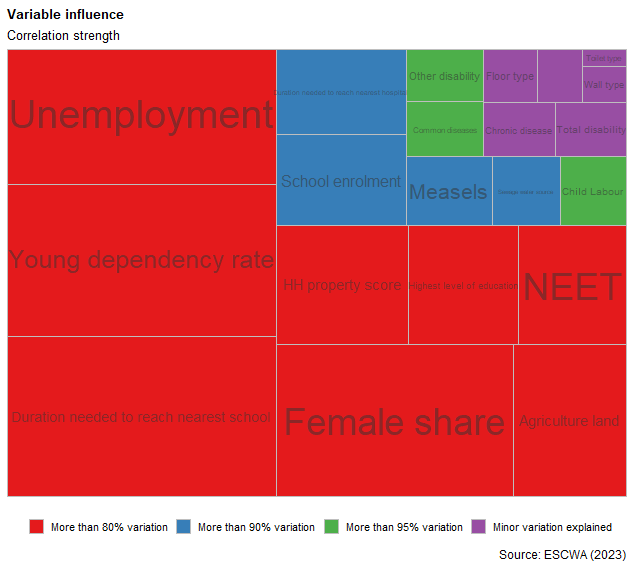
\includegraphics[keepaspectratio]{images/clipboard-1794507113.png}}

\textbf{Lasso Regression: Variable Selection and Shrinkage}

While the previous section focused on explanatory power, another
approach examines the~\textbf{magnitude of variable coefficients}.
Suppose the score is now defined as:

\[
Score = 0.1X + 10Y
\]

Although~\emph{X}~has a much smaller coefficient, is it negligible? To
answer this, we use~\textbf{Lasso regression}\footnote{Tibshirani, R.
  (1996). Regression Shrinkage and Selection via the lasso. Journal of
  the Royal Statistical Society. Series B (methodological), 267-288.}, a
technique that penalizes the inclusion of less important variables.

As mentioned earlier, Social Assistance programmes relied on the
estimation of the Proxy Mean Test that ~is defined though formulas like
the following:

\[
PMT = Y = β₀ + β₁X₁ + β₂X₂ + ... + βₙXₙ
\]

In the formula, the \emph{β} correspond to the weights and the \emph{X}
to the variables ~identified ad conceptually relevant from the social
registry ~and/or surveys where applicants provide information about
their socioeconomic variables.

~If the variables are transformed by a constant scalar: ~\[
 z_i=β_i x_i
 \] ~Then, the PMT becomes: ~\[
 PMT=β_0+α_1 z_1+α_2 z_2+α_3 z_3+⋯+α_N z_N
 \] ~Where \[α_1=α_2=⋯=α_N=1\]

So, in this second regression all the coefficients must be 1, and it
will be used as a benchmark for the Lasso regression. The linear
regression exercise is to calculate the values of \[β_0,β_1, … β_N\]
that minimize the sum of squared errors: \[
min┬(β_0,β_1,… β_N )⁡〖(Y-β_0-β_1 X_1-〖...- β〗_N X_N )^2 〗
\] Now, assume that having values of β different than 0 will cost. So
you also want to include that in the minimization exercise: \[
min┬(β_0,β_1,… β_N )⁡〖(Y-β_0-β_1 X_1-β_2 X_2-…-β_N X_N )^2+λ(|β_1 |+|β_2 |+⋯ +|β_N |)〗
\]

Hence, if \emph{λ=0}, this will be a typical ordinary least square; in
contrast, if \emph{λ=∞}, all \emph{β} will be 0 due to the high costs
associated in having them. Thus, by increasing \emph{λ} slowly, the
method begins to tell what the most important variables are, and there
are even some technical criteria, to explain what is the best \emph{λ}
that explains Y by using the least number of variables. Therefore, this
exercise not only allows to remove those variables that are less
meaningful, but also readjust the weights so that with fewer variables,
the scores can still be properly forecasted. In the script, Lasso
regression is estimated by determining the optimal lambda through a
cross-validation exercise, which is a standard approach in machine
learning. This is done using the \texttt{cv.glmnet} function, which
performs cross-validation to select the lambda value that minimizes
prediction error. The overall process involves: Running Lasso regression
across a range of lambda values, evaluating model performance (typically
via cross-validation), Selecting the lambda with the lowest
cross-validated error, analyzing the resulting coefficients to identify
redundant variables.

\begin{Shaded}
\begin{Highlighting}[]
\CommentTok{\# 4.5| Redundant Variable Analysis Using Lasso Regression }

\CommentTok{\# Create design matrix X for predictors (automatically handles factors/dummies)}
\NormalTok{X }\OtherTok{\textless{}{-}} \FunctionTok{model.matrix}\NormalTok{(score }\SpecialCharTok{\textasciitilde{}}\NormalTok{ ., TestingData)}

\CommentTok{\# Extract target variable}
\NormalTok{y }\OtherTok{\textless{}{-}}\NormalTok{ TestingData}\SpecialCharTok{$}\NormalTok{score }

\CommentTok{\# Set unconstrained bounds for LASSO coefficients}
\NormalTok{lb }\OtherTok{\textless{}{-}} \FunctionTok{rep}\NormalTok{(}\SpecialCharTok{{-}}\ConstantTok{Inf}\NormalTok{, }\FunctionTok{length}\NormalTok{(}\FunctionTok{colnames}\NormalTok{(X)))}
\NormalTok{ub }\OtherTok{\textless{}{-}} \FunctionTok{rep}\NormalTok{(}\ConstantTok{Inf}\NormalTok{, }\FunctionTok{length}\NormalTok{(}\FunctionTok{colnames}\NormalTok{(X)))}


\CommentTok{\# Estimate optimal lambda via cross{-}validated LASSO}

\NormalTok{cv\_las1 }\OtherTok{=} \FunctionTok{cv.glmnet}\NormalTok{(}\AttributeTok{x =}\NormalTok{ X, }\AttributeTok{y =}\NormalTok{ y, }\AttributeTok{lower.limits =}\NormalTok{ lb, }\AttributeTok{upper.limits =}\NormalTok{ ub)}
\NormalTok{lambda }\OtherTok{=}\NormalTok{ cv\_las1}\SpecialCharTok{$}\NormalTok{lambda.min  }\CommentTok{\# Best lambda minimizing CV error}


\CommentTok{\# Fit LASSO model with optimal lambda}
\NormalTok{las1 }\OtherTok{=} \FunctionTok{glmnet}\NormalTok{(}\AttributeTok{x =}\NormalTok{ X, }\AttributeTok{y =}\NormalTok{ y, }\AttributeTok{lower.limits =}\NormalTok{ lb, }\AttributeTok{upper.limits =}\NormalTok{ ub, }\AttributeTok{lambda =}\NormalTok{ lambda)}

\CommentTok{\# Extract coefficients and zero out small ones (\textless{} 0.05)}
\NormalTok{c.fit1 }\OtherTok{=} \FunctionTok{coef}\NormalTok{(las1) }\SpecialCharTok{\%\textgreater{}\%} \FunctionTok{as.matrix}\NormalTok{() }\SpecialCharTok{\%\textgreater{}\%} \FunctionTok{as.data.frame}\NormalTok{()}
\FunctionTok{colnames}\NormalTok{(c.fit1) }\OtherTok{=} \FunctionTok{c}\NormalTok{(}\StringTok{\textquotesingle{}Coefficient\textquotesingle{}}\NormalTok{)}
\NormalTok{namesVar }\OtherTok{=} \FunctionTok{rownames}\NormalTok{(c.fit1)}
\NormalTok{c.fit1}\SpecialCharTok{$}\NormalTok{Coefficient[}\FunctionTok{abs}\NormalTok{(c.fit1}\SpecialCharTok{$}\NormalTok{Coefficient) }\SpecialCharTok{\textless{}} \FloatTok{0.05}\NormalTok{] }\OtherTok{=} \DecValTok{0}  \CommentTok{\# Threshold}
\end{Highlighting}
\end{Shaded}

Once the optimal lambda is identified, the model is estimated and the
corresponding coefficients are examined. In the Nemey dataset, there are
no coefficients that are exactly zero for the optimized lambda, but some
are small enough to be considered negligible. These variables may not
contribute significantly to the model and could be candidates for
exclusion, ``redundant variables''. To run the exercise testing
different values of \emph{λ} (lambda)---also known as the lambda
tolerance or optimal lambda multiplier---the code iterates through the
chunk below and saves the results for each lambda value. Each lambda
corresponds to a different model configuration:

\begin{itemize}
\item
  Smaller \emph{λ} → Low bias, high variance: The model fits the
  training data well but may overfit.
\item
  Larger λ → High bias, low variance: The model is simpler with fewer
  variables, but it may underfit.
\end{itemize}

By plotting the variables selected at each lambda level, we can observe
which variables consistently drop out of the model as regularization
increases. These are likely to be the less informative or redundant
variables. More details and analytical graphs are available in the
script.

\emph{Figure 4.2 graph identifying potential variables to remove}

\pandocbounded{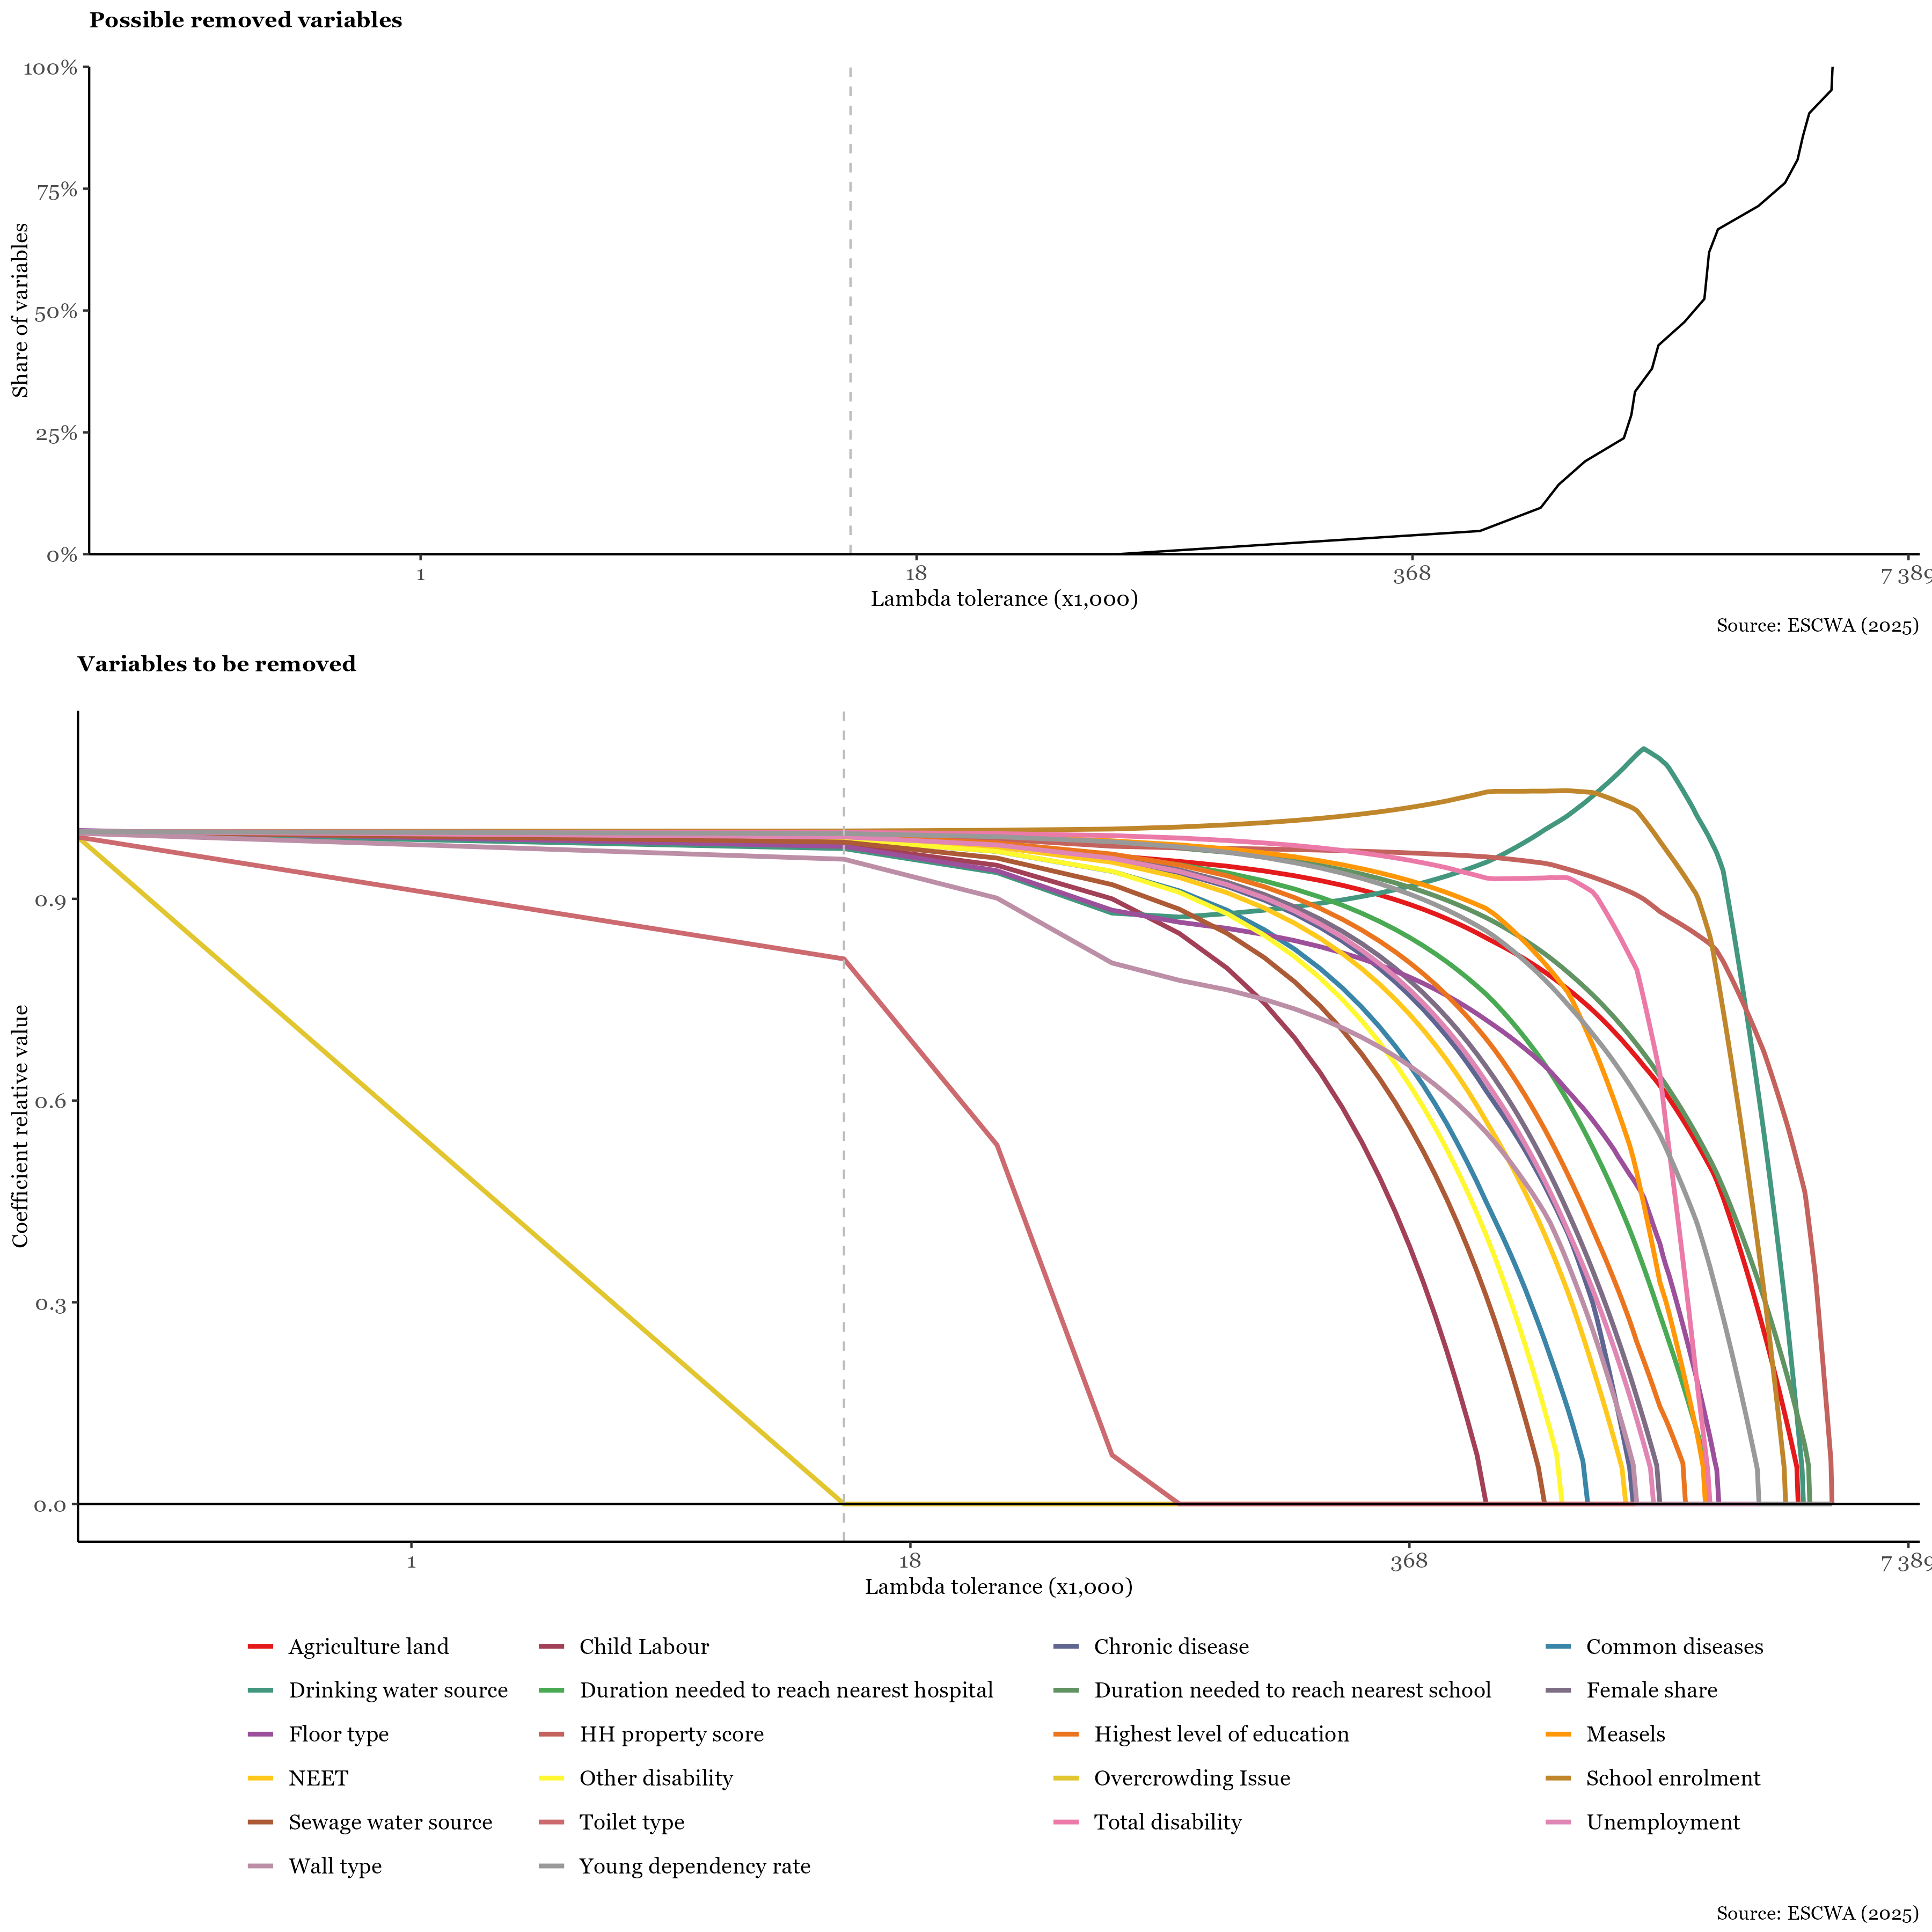
\includegraphics[keepaspectratio]{images/clipboard-4218109163.png}}

\subsection{5. Coverage evaluation}\label{coverage-evaluation}

The third stage of the framework focuses on identifying inclusion and
exclusion errors. On one hand, it analyzes the characteristics of
current beneficiaries to flag individuals whose circumstances may have
changed, suggesting they could be removed from the programme or
transferred to a different one. On the other hand, it identifies
individuals who may meet the eligibility criteria (or are likely to meet
them soon) but are not currently enrolled. This dual approach enables
policymakers to optimize resource allocation and assess whether outreach
efforts should be intensified to improve enrollment effectiveness.

This stage produces three key outputs: Indicators that help identify
potential beneficiaries, geographical areas where a higher concentration
of households meet the eligibility criteria and Insights into targeting
and eligibility processes, highlighting areas where inclusion of less
vulnerable households may need to be addressed.

To conduct this analysis, it is essential to have data on the same
variables for both beneficiaries and non-beneficiaries, including
applicants who were not selected. However, some programmes do not
collect complete information from non-applicants. In such cases, machine
learning techniques can be employed to impute missing values. Still, the
success of the analysis heavily depends on the availability of a
comprehensive dataset covering both groups.

To detect inclusion and exclusion errors the strategies are straight
forward recalculating scores and compare theoretical beneficiaries with
actual programme decisions whether the selection is via threshold -
households below certain score- or quota selection - ranking households
and selecting certain number of households as illustrated in Figure 5.1

\emph{Figure 5.1 methods to select beneficiaries.}

\pandocbounded{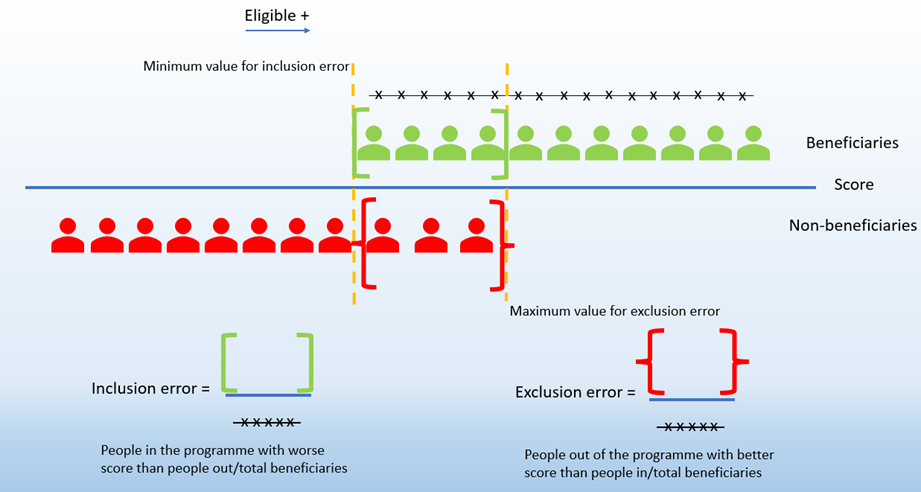
\includegraphics[keepaspectratio]{images/clipboard-1260681801.png}}

If desired, based on the inclusion and exclusion errors identified
earlier in the chapter, a clustering exercise is recommended but not
detailed in this manual. For inclusion errors, clustering highlights the
key variables that contributed to individuals receiving benefits despite
not qualifying based on their score. Although, this clustering approach
differs from the explanation below as it includes all variables and
could incorporate social workers' assessments (in case the programme has
information about it), the technical process is the same.

\subsubsection{\texorpdfstring{\textbf{Threshold-based
selection}}{Threshold-based selection}}\label{threshold-based-selection}

Let's consider the threshold as a method for selecting beneficiaries.
The first step is to identify a new category of beneficiaries, referred
to as \emph{theoretical beneficiaries}. Members are classified as
theoretical beneficiaries if their score is greater than or equal to 40.
To identify inclusion and exclusion errors, we compare the beneficiary
status provided earlier in the dataset with the newly defined
theoretical beneficiaries. The key section of the code is:

\begin{Shaded}
\begin{Highlighting}[]

\NormalTok{finalData}\OtherTok{=}\NormalTok{ finalData }\SpecialCharTok{\%\textgreater{}\%} 
  \FunctionTok{mutate}\NormalTok{(}
    \AttributeTok{theo\_beneficiary =} \FunctionTok{if\_else}\NormalTok{(score}\SpecialCharTok{\textgreater{}=} \DecValTok{40}\NormalTok{, }\StringTok{"Yes"}\NormalTok{, }\StringTok{"No"}\NormalTok{)}
\NormalTok{  )}
\end{Highlighting}
\end{Shaded}

Based on this threshold analysis, we compare real beneficiaries with
theoretical ones. This comparison can be further analyzed by grouping
data according to categorical variables, such as gender, as illustrated
in the graph below. For example, among all female real beneficiaries,
only 75\% were also theoretical beneficiaries. Additionally, less than
8\% of those who were not theoretical beneficiaries were still included
as beneficiaries. The code introduces inclusion and exclusion errors by
relevant variables such as gender, and also generates a hypothetical map
showing the distribution of theoretical beneficiaries.

\emph{Figure 5.2 Example of inclusion/exclusion errors descriptive
statistics by gender}

\pandocbounded{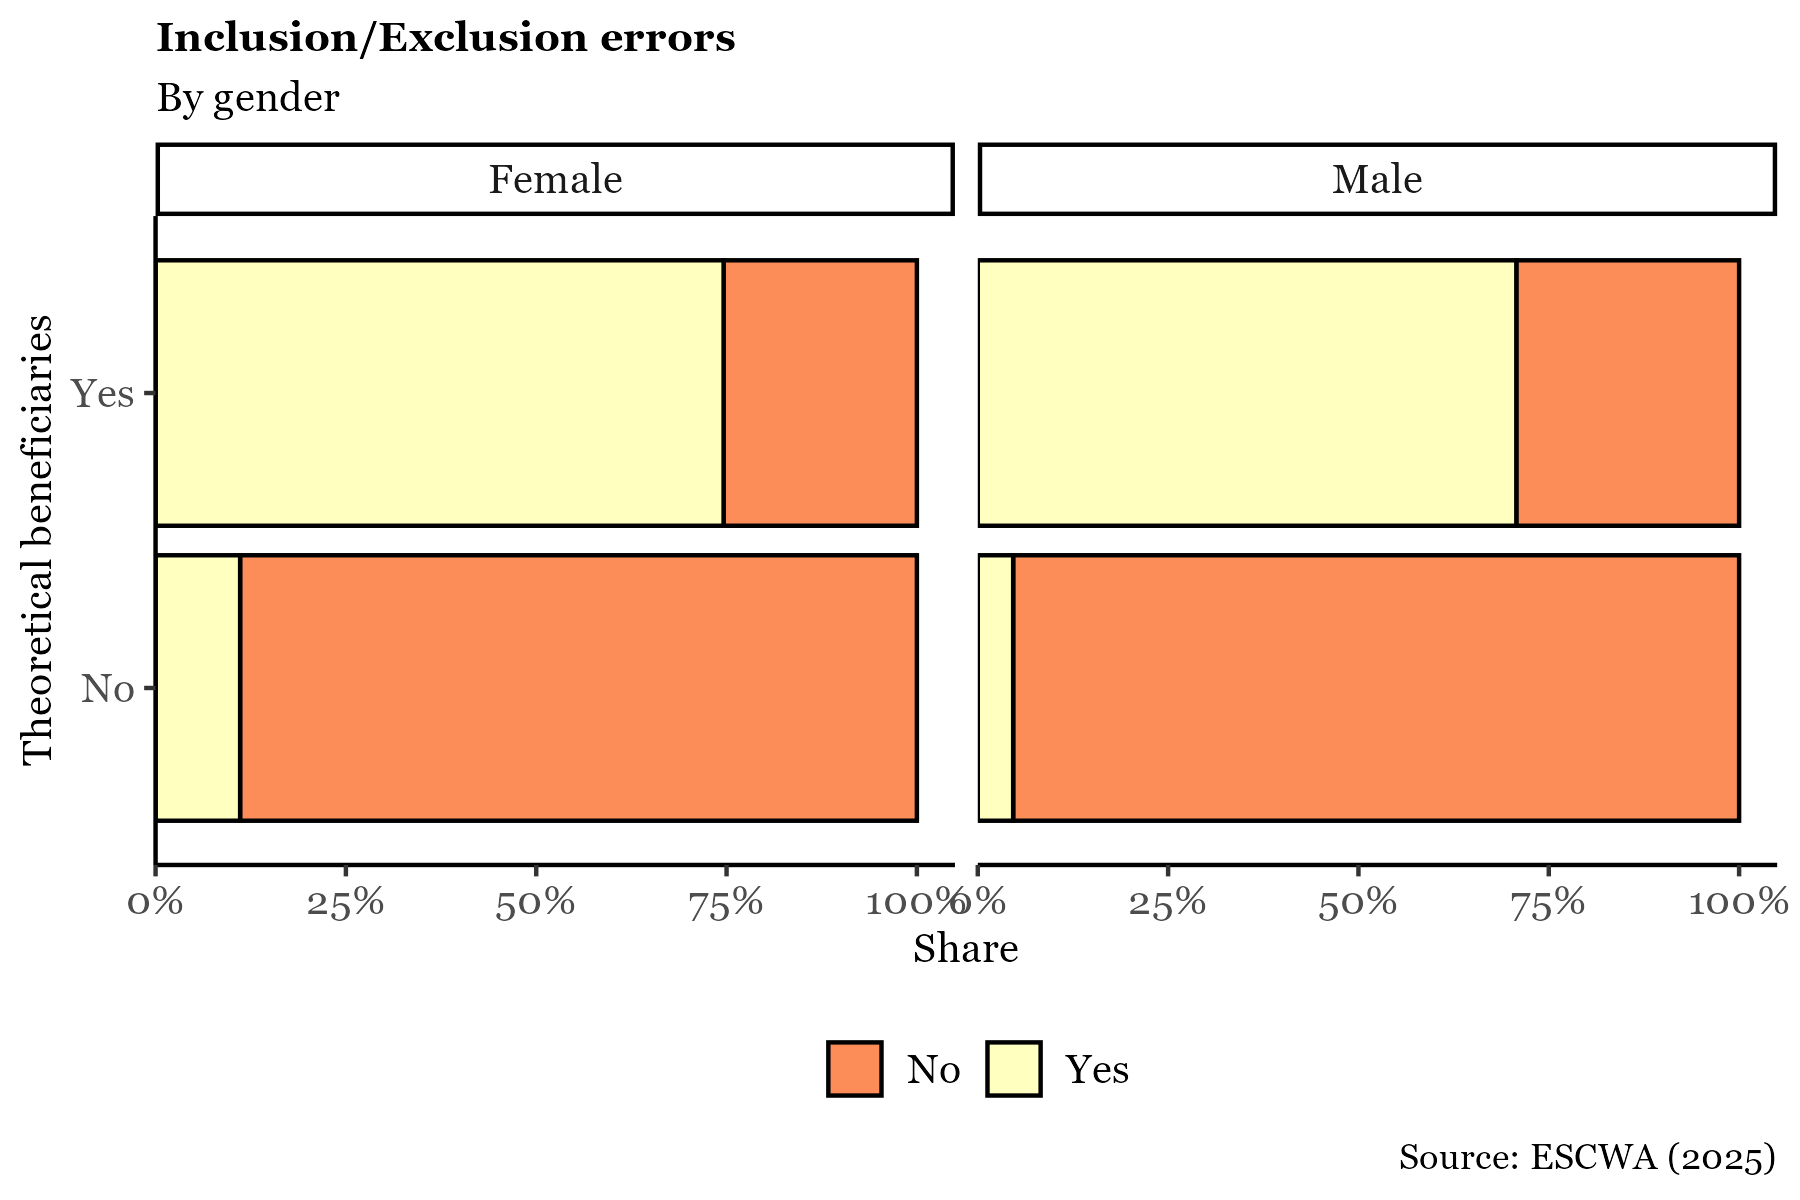
\includegraphics[keepaspectratio]{images/clipboard-2131893230.png}}

\subsubsection{\texorpdfstring{\textbf{Ranking based selection: Fixed
number of individuals/households
selection}}{Ranking based selection: Fixed number of individuals/households selection}}\label{ranking-based-selection-fixed-number-of-individualshouseholds-selection}

When beneficiary selection is based on a \textbf{fixed number of
individuals ranked by score}, the process differs from using a
predetermined score threshold. In this case, inclusion and exclusion
errors cannot be defined by comparing scores against a fixed value.
Instead, the strategy must adapt to the ranking-based selection.

\begin{itemize}
\item
  \textbf{Exclusion error} refers to individuals who were not selected
  as beneficiaries, yet have scores above the minimum score of those who
  were selected. This implies that some more vulnerable individuals were
  left out.
\item
  \textbf{Inclusion error} refers to individuals who were selected as
  beneficiaries, yet have scores below the maximum score found among the
  non-beneficiaries. This suggests that some less vulnerable individuals
  were included.

  One way to assess this visually is by comparing score distributions.
  Exclusion errors occur when individuals in the non-beneficiary group
  (left side of the distribution) have scores above the minimum score
  observed in the beneficiary group. In contrast, inclusion errors occur
  when beneficiaries have scores below the maximum score observed in the
  non-beneficiary group.
\end{itemize}

\begin{Shaded}
\begin{Highlighting}[]
\NormalTok{error\_metrics }\OtherTok{\textless{}{-}}\NormalTok{ finalData }\SpecialCharTok{\%\textgreater{}\%}
  \FunctionTok{drop\_na}\NormalTok{(Beneficiaries, Governorate) }\SpecialCharTok{\%\textgreater{}\%}
  \FunctionTok{group\_by}\NormalTok{(Governorate) }\SpecialCharTok{\%\textgreater{}\%}
  \FunctionTok{summarise}\NormalTok{(}
    \CommentTok{\# Define thresholds}
    \AttributeTok{min\_inc =} \FunctionTok{min}\NormalTok{(score[Beneficiaries }\SpecialCharTok{==} \StringTok{"Yes"}\NormalTok{], }\AttributeTok{na.rm =} \ConstantTok{TRUE}\NormalTok{),}
    \AttributeTok{max\_excl =} \FunctionTok{max}\NormalTok{(score[Beneficiaries }\SpecialCharTok{==} \StringTok{"No"}\NormalTok{], }\AttributeTok{na.rm =} \ConstantTok{TRUE}\NormalTok{),}
    
    \CommentTok{\# Inclusion error: beneficiaries with score below max score of non{-}beneficiaries}
    \AttributeTok{incl\_cases =} \FunctionTok{sum}\NormalTok{(Beneficiaries }\SpecialCharTok{==} \StringTok{"Yes"} \SpecialCharTok{\&}\NormalTok{ score }\SpecialCharTok{\textless{}}\NormalTok{ max\_excl, }\AttributeTok{na.rm =} \ConstantTok{TRUE}\NormalTok{),}
    \AttributeTok{benefiting =} \FunctionTok{sum}\NormalTok{(Beneficiaries }\SpecialCharTok{==} \StringTok{"Yes"}\NormalTok{, }\AttributeTok{na.rm =} \ConstantTok{TRUE}\NormalTok{),}
    
    \CommentTok{\# Exclusion error: non{-}beneficiaries with score above min score of beneficiaries}
    \AttributeTok{excl\_cases =} \FunctionTok{sum}\NormalTok{(Beneficiaries }\SpecialCharTok{==} \StringTok{"No"} \SpecialCharTok{\&}\NormalTok{ score }\SpecialCharTok{\textgreater{}}\NormalTok{ min\_inc, }\AttributeTok{na.rm =} \ConstantTok{TRUE}\NormalTok{),}
    \AttributeTok{no\_benefiting =} \FunctionTok{sum}\NormalTok{(Beneficiaries }\SpecialCharTok{==} \StringTok{"No"}\NormalTok{, }\AttributeTok{na.rm =} \ConstantTok{TRUE}\NormalTok{),}
    
    \AttributeTok{.groups =} \StringTok{"drop"}
\NormalTok{  ) }\SpecialCharTok{\%\textgreater{}\%}
  \FunctionTok{mutate}\NormalTok{(}
    \AttributeTok{incl\_error =}\NormalTok{ incl\_cases }\SpecialCharTok{/}\NormalTok{ benefiting,}
    \AttributeTok{exc\_error =}\NormalTok{ excl\_cases }\SpecialCharTok{/}\NormalTok{ no\_benefiting}
\NormalTok{  ) }\SpecialCharTok{\%\textgreater{}\%}
\NormalTok{  dplyr}\SpecialCharTok{::}\FunctionTok{select}\NormalTok{(Governorate, incl\_error, exc\_error)}


\CommentTok{\# Split into separate datasets}
\NormalTok{temp\_inc\_final }\OtherTok{\textless{}{-}}\NormalTok{ error\_metrics }\SpecialCharTok{\%\textgreater{}\%}\NormalTok{ dplyr}\SpecialCharTok{::}\FunctionTok{select}\NormalTok{(Governorate, incl\_error)}
\NormalTok{temp\_exc\_final }\OtherTok{\textless{}{-}}\NormalTok{ error\_metrics }\SpecialCharTok{\%\textgreater{}\%}\NormalTok{ dplyr}\SpecialCharTok{::}\FunctionTok{select}\NormalTok{(Governorate, exc\_error)}
\end{Highlighting}
\end{Shaded}

Under this definition, inclusion error may appear disproportionately
high. This needs to be interpreted carefully, especially since the score
is a relative measure of vulnerability, and many applicants, whether
selected or not, may still be highly vulnerable. For example, some
individuals not selected due to other criteria (such as social worker
evaluations) may still have high levels of vulnerability.

Therefore, using the maximum score of non-beneficiaries as a benchmark
for inclusion error may not be ideal. It is often recommended to assess
inclusion errors against external vulnerability indicators, such as the
poverty line, which are not relative to the sample.

Maps can also be produced using these definitions, as shown in the code.

\emph{Figure 5.3 Inclusion Exclusion errors scores' density plot}

\pandocbounded{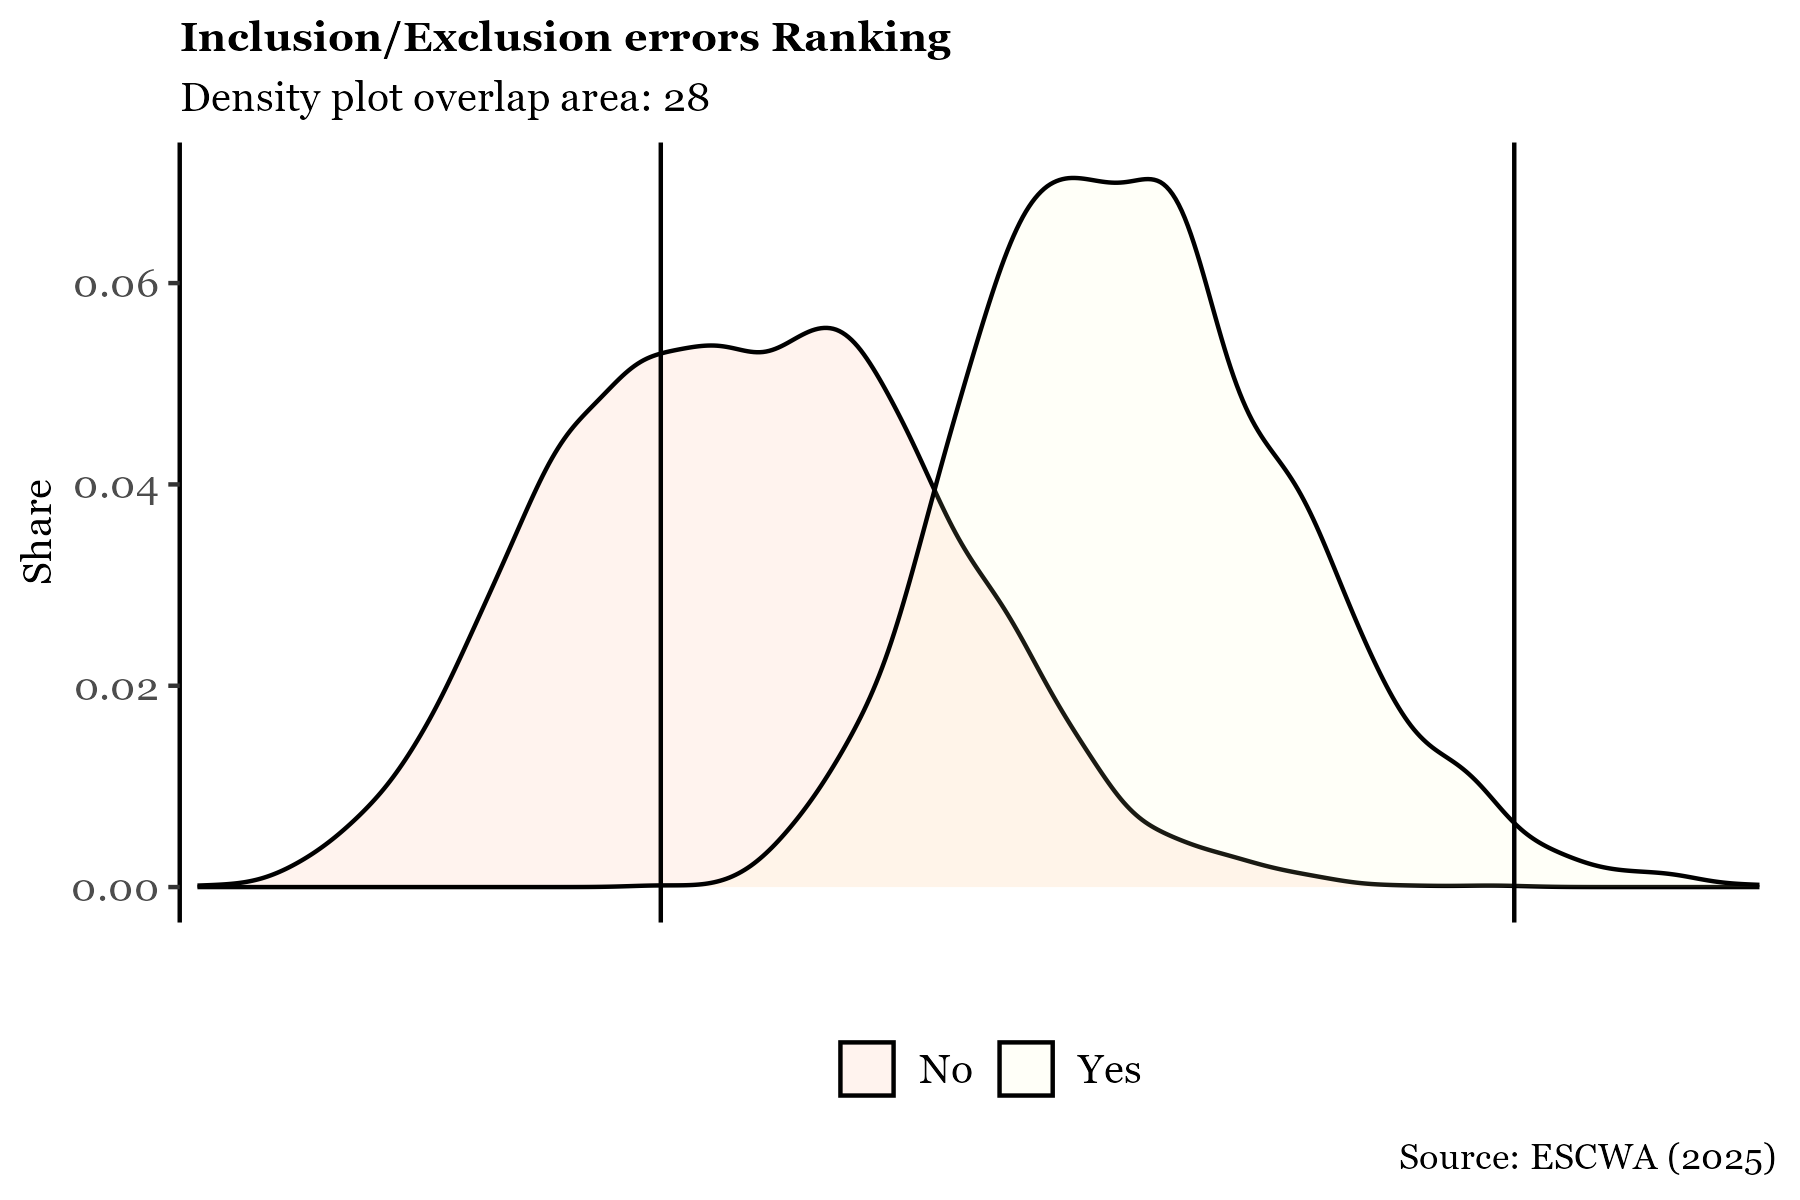
\includegraphics[keepaspectratio]{images/clipboard-2153169490.png}}

\subsection{\texorpdfstring{\textbf{Annex: Missing
values}}{Annex: Missing values}}\label{annex-missing-values}

To address missing values and statistically compare the variables
reported by applicants with those predicted based on other available
information, a decision tree model can be employed. This approach is
particularly useful when the data is self-reported rather than observed
directly, as applicants may tend to overstate their vulnerability to
increase their chances of receiving benefits. From an analytical
perspective, it is also valuable to compare the actual vulnerability
score with the score estimated statistically. To do this, each variable
is predicted individually using the remaining data, and a new
``estimated'' vulnerability score is calculated. This score is then used
to compute the Proxy Means Test (PMT), as illustrated below.

\begin{Shaded}
\begin{Highlighting}[]

\NormalTok{PMTIndicators1}\OtherTok{=}\NormalTok{PMTIndicators }\CommentTok{\# to create}
\NormalTok{PMTIndicators2}\OtherTok{=}\NormalTok{PMTIndicators }\CommentTok{\# to update}

\NormalTok{var\_types }\OtherTok{\textless{}{-}} \FunctionTok{list}\NormalTok{(}
  \AttributeTok{discrete =} \FunctionTok{c}\NormalTok{(}
    \StringTok{"var\_overcrowdingIssue"}\NormalTok{, }\StringTok{"var\_Wall\_type"}\NormalTok{, }\StringTok{"var\_Floor\_type"}\NormalTok{, }
    \StringTok{"var\_Toilet\_Type"}\NormalTok{, }\StringTok{"var\_Drinking\_water"}\NormalTok{, }\StringTok{"var\_sewage"}\NormalTok{,}
    \StringTok{"var\_AgriLand"}\NormalTok{, }\StringTok{"var\_chronic"}\NormalTok{, }\StringTok{"var\_duration\_hospital"}\NormalTok{,}
    \StringTok{"var\_duration\_school"}\NormalTok{, }\StringTok{"var\_NEET"}
\NormalTok{  ),}
  \AttributeTok{continuous =} \FunctionTok{c}\NormalTok{(}
    \StringTok{"var\_Property\_score"}\NormalTok{, }\StringTok{"var\_common"}\NormalTok{, }\StringTok{"var\_measels"}\NormalTok{,}
    \StringTok{"var\_tot\_disab"}\NormalTok{, }\StringTok{"var\_other\_disab"}\NormalTok{, }\StringTok{"var\_enrolment"}\NormalTok{,}
    \StringTok{"var\_high\_education\_rate"}\NormalTok{, }\StringTok{"var\_unemployment\_rate"}\NormalTok{,}
    \StringTok{"var\_child\_labour"}\NormalTok{, }\StringTok{"var\_female\_ratio"}\NormalTok{, }
    \StringTok{"var\_young\_dependency\_ratio"}
\NormalTok{  )}
\NormalTok{)}

\NormalTok{predict\_variable }\OtherTok{\textless{}{-}} \ControlFlowTok{function}\NormalTok{(var\_name, data, new\_data) \{}
  \CommentTok{\# Remove HHID and the target variable from predictors}
\NormalTok{  predictors }\OtherTok{\textless{}{-}}\NormalTok{ data }\SpecialCharTok{\%\textgreater{}\%}\NormalTok{ dplyr}\SpecialCharTok{::}\FunctionTok{select}\NormalTok{(}\SpecialCharTok{{-}}\NormalTok{HHID, }\SpecialCharTok{{-}}\FunctionTok{all\_of}\NormalTok{(var\_name))}
  
  \ControlFlowTok{if}\NormalTok{ (var\_name }\SpecialCharTok{\%in\%}\NormalTok{ var\_types}\SpecialCharTok{$}\NormalTok{discrete) \{}
    \CommentTok{\# For discrete variables {-} classification tree}
\NormalTok{    formula }\OtherTok{\textless{}{-}} \FunctionTok{as.formula}\NormalTok{(}\FunctionTok{paste}\NormalTok{(}\StringTok{"factor("}\NormalTok{, var\_name, }\StringTok{") \textasciitilde{} ."}\NormalTok{))}
\NormalTok{    tree }\OtherTok{\textless{}{-}} \FunctionTok{rpart}\NormalTok{(formula, }\AttributeTok{data =}\NormalTok{ data }\SpecialCharTok{\%\textgreater{}\%}\NormalTok{ dplyr}\SpecialCharTok{::}\FunctionTok{select}\NormalTok{(}\SpecialCharTok{{-}}\NormalTok{HHID), }
                  \AttributeTok{method =} \StringTok{"class"}\NormalTok{)}
\NormalTok{    pred }\OtherTok{\textless{}{-}} \FunctionTok{as.numeric}\NormalTok{(}\FunctionTok{as.character}\NormalTok{(}\FunctionTok{predict}\NormalTok{(tree, new\_data, }\AttributeTok{type =} \StringTok{"class"}\NormalTok{)))}
\NormalTok{  \} }\ControlFlowTok{else}\NormalTok{ \{}
    \CommentTok{\# For continuous variables {-} regression tree}
\NormalTok{    formula }\OtherTok{\textless{}{-}} \FunctionTok{as.formula}\NormalTok{(}\FunctionTok{paste}\NormalTok{(var\_name, }\StringTok{"\textasciitilde{} ."}\NormalTok{))}
\NormalTok{    tree }\OtherTok{\textless{}{-}} \FunctionTok{rpart}\NormalTok{(formula, }\AttributeTok{data =}\NormalTok{ data }\SpecialCharTok{\%\textgreater{}\%}\NormalTok{ dplyr}\SpecialCharTok{::}\FunctionTok{select}\NormalTok{(}\SpecialCharTok{{-}}\NormalTok{HHID), }
                  \AttributeTok{method =} \StringTok{"anova"}\NormalTok{)}
\NormalTok{    pred }\OtherTok{\textless{}{-}} \FunctionTok{predict}\NormalTok{(tree, new\_data)}
\NormalTok{  \}}
  
  \FunctionTok{return}\NormalTok{(pred)}
\NormalTok{\}}


\ControlFlowTok{for}\NormalTok{ (var }\ControlFlowTok{in} \FunctionTok{c}\NormalTok{(var\_types}\SpecialCharTok{$}\NormalTok{discrete, var\_types}\SpecialCharTok{$}\NormalTok{continuous)) \{}
\NormalTok{  PMTIndicators2[[var]] }\OtherTok{\textless{}{-}} \FunctionTok{predict\_variable}\NormalTok{(var, PMTIndicators1, PMTIndicators1)}
\NormalTok{\}}

\NormalTok{SCORING2 }\OtherTok{=}\NormalTok{ PMTIndicators2 }\SpecialCharTok{\%\textgreater{}\%} 
  \FunctionTok{mutate}\NormalTok{(}
    \AttributeTok{s\_var\_overcrowdingIssue=}\NormalTok{(}\DecValTok{1}\SpecialCharTok{/}\DecValTok{6}\NormalTok{)}\SpecialCharTok{*}\NormalTok{(}\DecValTok{1}\SpecialCharTok{/}\DecValTok{7}\NormalTok{)}\SpecialCharTok{*}\NormalTok{var\_overcrowdingIssue, }\CommentTok{\# the value next to each variable is its weight. in this case we specified the weight but in other cases we have to stick to the weight given}
    \AttributeTok{s\_var\_Wall=}\NormalTok{(}\DecValTok{1}\SpecialCharTok{/}\DecValTok{6}\NormalTok{)}\SpecialCharTok{*}\NormalTok{(}\DecValTok{1}\SpecialCharTok{/}\DecValTok{7}\NormalTok{)}\SpecialCharTok{*}\NormalTok{var\_Wall\_type,}
    \AttributeTok{s\_var\_Floor=}\NormalTok{(}\DecValTok{1}\SpecialCharTok{/}\DecValTok{6}\NormalTok{)}\SpecialCharTok{*}\NormalTok{(}\DecValTok{1}\SpecialCharTok{/}\DecValTok{7}\NormalTok{)}\SpecialCharTok{*}\NormalTok{var\_Floor\_type,}
    \AttributeTok{s\_var\_Toilet=}\NormalTok{(}\DecValTok{1}\SpecialCharTok{/}\DecValTok{6}\NormalTok{)}\SpecialCharTok{*}\NormalTok{(}\DecValTok{1}\SpecialCharTok{/}\DecValTok{7}\NormalTok{)}\SpecialCharTok{*}\NormalTok{var\_Toilet\_Type,}
    \AttributeTok{s\_var\_DrinkWater=}\NormalTok{(}\DecValTok{1}\SpecialCharTok{/}\DecValTok{6}\NormalTok{)}\SpecialCharTok{*}\NormalTok{(}\DecValTok{1}\SpecialCharTok{/}\DecValTok{7}\NormalTok{)}\SpecialCharTok{*}\NormalTok{var\_Drinking\_water,}
    \AttributeTok{s\_var\_Sewage=}\NormalTok{(}\DecValTok{1}\SpecialCharTok{/}\DecValTok{6}\NormalTok{)}\SpecialCharTok{*}\NormalTok{(}\DecValTok{1}\SpecialCharTok{/}\DecValTok{7}\NormalTok{)}\SpecialCharTok{*}\NormalTok{var\_sewage,}
    
    \AttributeTok{s\_var\_Property=}\NormalTok{(}\DecValTok{1}\SpecialCharTok{/}\DecValTok{2}\NormalTok{)}\SpecialCharTok{*}\NormalTok{(}\DecValTok{1}\SpecialCharTok{/}\DecValTok{7}\NormalTok{)}\SpecialCharTok{*}\NormalTok{var\_Property\_score,}
    \AttributeTok{s\_var\_agriLand=}\NormalTok{(}\DecValTok{1}\SpecialCharTok{/}\DecValTok{2}\NormalTok{)}\SpecialCharTok{*}\NormalTok{(}\DecValTok{1}\SpecialCharTok{/}\DecValTok{7}\NormalTok{)}\SpecialCharTok{*}\NormalTok{var\_AgriLand,}
    
    \AttributeTok{s\_var\_chronic=}\NormalTok{(}\DecValTok{1}\SpecialCharTok{/}\DecValTok{6}\NormalTok{)}\SpecialCharTok{*}\NormalTok{(}\DecValTok{1}\SpecialCharTok{/}\DecValTok{7}\NormalTok{)}\SpecialCharTok{*}\NormalTok{var\_chronic,}
    \AttributeTok{s\_var\_common=}\NormalTok{(}\DecValTok{1}\SpecialCharTok{/}\DecValTok{6}\NormalTok{)}\SpecialCharTok{*}\NormalTok{(}\DecValTok{1}\SpecialCharTok{/}\DecValTok{7}\NormalTok{)}\SpecialCharTok{*}\NormalTok{var\_common,}
    \AttributeTok{s\_var\_measels=}\NormalTok{(}\DecValTok{1}\SpecialCharTok{/}\DecValTok{6}\NormalTok{)}\SpecialCharTok{*}\NormalTok{(}\DecValTok{1}\SpecialCharTok{/}\DecValTok{7}\NormalTok{)}\SpecialCharTok{*}\NormalTok{var\_measels,}
    \AttributeTok{s\_var\_totdisab=}\NormalTok{(}\DecValTok{1}\SpecialCharTok{/}\DecValTok{6}\NormalTok{)}\SpecialCharTok{*}\NormalTok{(}\DecValTok{1}\SpecialCharTok{/}\DecValTok{7}\NormalTok{)}\SpecialCharTok{*}\NormalTok{var\_tot\_disab,}
    \AttributeTok{s\_var\_otherdisab=}\NormalTok{(}\DecValTok{1}\SpecialCharTok{/}\DecValTok{6}\NormalTok{)}\SpecialCharTok{*}\NormalTok{(}\DecValTok{1}\SpecialCharTok{/}\DecValTok{7}\NormalTok{)}\SpecialCharTok{*}\NormalTok{var\_other\_disab,}
    \AttributeTok{s\_var\_durationHospital=}\NormalTok{(}\DecValTok{1}\SpecialCharTok{/}\DecValTok{6}\NormalTok{)}\SpecialCharTok{*}\NormalTok{(}\DecValTok{1}\SpecialCharTok{/}\DecValTok{7}\NormalTok{)}\SpecialCharTok{*}\NormalTok{var\_duration\_hospital,}
    
    \AttributeTok{s\_var\_enrolment=}\NormalTok{(}\DecValTok{1}\SpecialCharTok{/}\DecValTok{3}\NormalTok{)}\SpecialCharTok{*}\NormalTok{(}\DecValTok{1}\SpecialCharTok{/}\DecValTok{7}\NormalTok{)}\SpecialCharTok{*}\NormalTok{var\_enrolment,}
    \AttributeTok{s\_var\_higheducation=}\NormalTok{(}\DecValTok{1}\SpecialCharTok{/}\DecValTok{3}\NormalTok{)}\SpecialCharTok{*}\NormalTok{(}\DecValTok{1}\SpecialCharTok{/}\DecValTok{7}\NormalTok{)}\SpecialCharTok{*}\NormalTok{var\_high\_education\_rate,}
    \AttributeTok{s\_var\_durationSchool=}\NormalTok{(}\DecValTok{1}\SpecialCharTok{/}\DecValTok{3}\NormalTok{)}\SpecialCharTok{*}\NormalTok{(}\DecValTok{1}\SpecialCharTok{/}\DecValTok{7}\NormalTok{)}\SpecialCharTok{*}\NormalTok{var\_duration\_school,}
    
    \AttributeTok{s\_var\_NEET=}\NormalTok{(}\DecValTok{1}\SpecialCharTok{/}\DecValTok{3}\NormalTok{)}\SpecialCharTok{*}\NormalTok{(}\DecValTok{1}\SpecialCharTok{/}\DecValTok{7}\NormalTok{)}\SpecialCharTok{*}\NormalTok{var\_NEET,}
    \AttributeTok{s\_var\_unemp=}\NormalTok{(}\DecValTok{1}\SpecialCharTok{/}\DecValTok{3}\NormalTok{)}\SpecialCharTok{*}\NormalTok{(}\DecValTok{1}\SpecialCharTok{/}\DecValTok{7}\NormalTok{)}\SpecialCharTok{*}\NormalTok{var\_unemployment\_rate,}
    \AttributeTok{s\_var\_childLabour=}\NormalTok{(}\DecValTok{1}\SpecialCharTok{/}\DecValTok{3}\NormalTok{)}\SpecialCharTok{*}\NormalTok{(}\DecValTok{1}\SpecialCharTok{/}\DecValTok{7}\NormalTok{)}\SpecialCharTok{*}\NormalTok{var\_child\_labour,}
    
    \AttributeTok{s\_var\_female=}\NormalTok{(}\DecValTok{1}\SpecialCharTok{/}\DecValTok{2}\NormalTok{)}\SpecialCharTok{*}\NormalTok{(}\DecValTok{1}\SpecialCharTok{/}\DecValTok{7}\NormalTok{)}\SpecialCharTok{*}\NormalTok{var\_female\_ratio,}
    \AttributeTok{s\_var\_youngdependency=}\NormalTok{(}\DecValTok{1}\SpecialCharTok{/}\DecValTok{2}\NormalTok{)}\SpecialCharTok{*}\NormalTok{(}\DecValTok{1}\SpecialCharTok{/}\DecValTok{7}\NormalTok{)}\SpecialCharTok{*}\NormalTok{var\_young\_dependency\_ratio,}
    
    \AttributeTok{score2 =}\NormalTok{ s\_var\_overcrowdingIssue  }\SpecialCharTok{+}\NormalTok{ s\_var\_Wall }\SpecialCharTok{+}\NormalTok{ s\_var\_Floor }\SpecialCharTok{+}\NormalTok{  s\_var\_Toilet }\SpecialCharTok{+}\NormalTok{ s\_var\_DrinkWater }\SpecialCharTok{+}\NormalTok{ s\_var\_Sewage }\SpecialCharTok{+}\NormalTok{ s\_var\_Property }\SpecialCharTok{+}\NormalTok{ s\_var\_agriLand }\SpecialCharTok{+}\NormalTok{ s\_var\_chronic }\SpecialCharTok{+}\NormalTok{ s\_var\_common }\SpecialCharTok{+}\NormalTok{ s\_var\_measels }\SpecialCharTok{+}\NormalTok{ s\_var\_totdisab }\SpecialCharTok{+}\NormalTok{ s\_var\_otherdisab }\SpecialCharTok{+}
\NormalTok{      s\_var\_durationHospital }\SpecialCharTok{+}\NormalTok{ s\_var\_enrolment}\SpecialCharTok{+}\NormalTok{ s\_var\_higheducation }\SpecialCharTok{+}\NormalTok{ s\_var\_durationSchool }\SpecialCharTok{+}\NormalTok{ s\_var\_NEET }\SpecialCharTok{+}\NormalTok{  s\_var\_unemp }\SpecialCharTok{+}\NormalTok{ s\_var\_childLabour }\SpecialCharTok{+}\NormalTok{s\_var\_female }\SpecialCharTok{+}\NormalTok{  s\_var\_youngdependency )}\SpecialCharTok{\%\textgreater{}\%}
  \FunctionTok{drop\_na}\NormalTok{()}
\end{Highlighting}
\end{Shaded}


\end{document}
